%%%%%%%%%%%%%%%%%%%%%%%%%%%%%%%%%%%%%%%%%%%%%%%%%%%%%%%%%%%%%%%%%%%%%%
%% September 9, 2015
%%
%% JLAB-THY-15-xxxx
%%%%%%%%%%%%%%%%%%%%%%%%%%%%%%%%%%%%%%%%%%%%%%%%%%%%%%%%%%%%%%%%%%%%%%%
\documentclass[aps,prd,amsmath,preprint]{revtex4}

% \voffset 1cm

\usepackage[utf8]{inputenc}
\usepackage{enumerate}
\usepackage{amsmath,amssymb}
\usepackage{bm}
\usepackage{amscd}            % for extensible arrows (e.g., limits)
\usepackage{graphicx}
\usepackage{hhline,multirow}  % for nicer tables
\usepackage{dcolumn}          % Align table columns on decimal point
\usepackage{url}              % for URL addresses
\usepackage[colorlinks=true,linkcolor=blue]{hyperref}
\usepackage{color}

\newcommand{\mc}{\multicolumn}
\newcommand{\s}{\hspace*{.2cm}}
\newcommand{\tik}{\checkmark}

\preprint{JLAB-THY-15-xxxx}

\begin{document}

\title{Constraints on large-$x$ parton distributions from new \\
	weak boson production and deep-inelastic scattering data}

% \author{A.~Accardi$^{1,2}$,
%	L.~T.~Brady$^{2,3}$,
%%%	P.~J.~Ehlers$^{2,4}$,
%	C.~E.~Keppel$^2$,
%	W.~Melnitchouk$^2$
%	J.~F.~Owens$^5$,
%	Nobuo~Sato$^2$, ...}
%
% \affiliation{
% $^1$\mbox{Hampton University, Hampton, Virginia 23668} \\
% $^2$\mbox{Jefferson Lab, Newport News, Virginia 23606} \\
% $^3$\mbox{University of California, Santa Barbara, California 93106, USA} \\
%%% $^4$\mbox{University of Washington, Seattle, Washington 98195, USA} \\
% $^5$\mbox{Florida State University, Tallahassee, Florida 32306, USA} \\
% {\bf CTEQ-Jefferson Lab (CJ) Collaboration}\\
% }


\date{\today}

\begin{abstract}
We present a new set of leading twist parton distribution functions
(PDFs), which take advantage of developments in the theoretical
treatment of nuclear corrections as well as new data.
The analysis includes for the first time data on the free neutron
structure function from the BONuS experiment at Jefferson Lab,
and new charged lepton and $W$-boson asymmetry data from Fermilab,
which significantly reduce the uncertainty on the $d/u$ ratio at
large values of $x$.
\end{abstract}

\maketitle


%%%%%%%%%%%%%%%%%%%%%%%%%%%%%%%%%%%%%%%%%%%%%%%%%%%%%%%%%%%%%%%%%%%%%%%%%
\section{Introduction} {\color{red} [XXX to edit]}
\label{sec:intro}

... general intro ...

... what is new since CJ12 ...

$\bullet$
more complete/consistent/systematic treatment of nuclear corrections
esp. nucleon off-shell corrections

$\bullet$
impact of new $W$-boson asymmetry data on $d/u$ ratio

$\bullet$
inclusion of JLab (BONuS) data

$\bullet$
analysis of $\bar d - \bar u$ at large $x$ ... choose either
$\bar d/\bar u \to 1$ or 0 as $x \to 1$ ...

$\bullet$
S-ACOT scheme for heavy quarks

$\bullet$
LO fit

$\bullet$
$\alpha_s$ treatment



... In Sec.~\ref{sec:thy} we ...


% In the following section we describe the methodology involved in the
% fits, including the choices of data sets, the parametrizations used,
% and the treatment of nuclear and finite-$Q^2$ corrections.  We also
% discuss the treatment of the experimental errors and the resulting
% error PDF sets.  In Sec.~\ref{sec:results} we present an overview of
% the CJ12 PDF results, and compare these with results from other global
% fits.  Finally, in Sec.~\ref{sec:conclusion} we make some concluding
% remarks and outline plans for future work.  An appendix is provided
% which contains the initial parameter values for each of the PDF sets.


%%%%%%%%%%%%%%%%%%%%%%%%%%%%%%%%%%%%%%%%%%%%%%%%%%%%%%%%%%%%%%%%%%%%%%%%%
\section{Theoretical foundations}
\label{sec:thy}

In this section we present the theoretical framework that is used for
the CJ15 analysis.


% .......................................................................
\subsection{PDF parametrizations {\color{red} [XXX to edit]}}
\label{ssec:parametrizations}

$\bullet$
For the parametrization of the PDFs at the input scale $Q_0^2$,
a common form has been adopted for all parton species $f$,
%
\begin{equation}
xf(x,Q_0^2) = a_0 x^{a_1} (1-x)^{a_2} (1 + a_3 \sqrt{x} + a_4 x).
\label{eq:param}
\end{equation}   
%
This form applies to the valence distributions
  $xq_v \equiv x(q-\bar q)$, for $q=u$ and $d$,
the isoscalar and isovector sea quark distributions
  $x(\bar u + \bar d)$ and $x(\bar d - \bar u)$,
and the gluon distribution $xg$.
However, to allow for a more flexible parametrization of the valence
$d_v$ PDF in the large-$x$ region, we add in a small admixture of the
$u_v$ PDF,
%
\begin{equation}
d_v \rightarrow
    a_0^{d_v} \left( \frac{d_v}{a_0^{d_v}} + b\, x^c u_v \right),
\label{eq:du}
\end{equation}
%
with $b$ and $c$ as two additional parameters.
The result of this modification is that
	$d_v/u_v \to a_0^{d_v}\, b$ as $x \to 1$,
provided $a_2^{d_v} > a_2^{u_v}$, which is usually the case.
A finite, nonzero value of this ratio is indeed expected in several
nonperturbative models of hadron structure \cite{FJ75, MT96, HR10}.
It is also required from a purely practical point of view, as it avoids
potentially large biases on the $d$-quark PDF central value \cite{CJ11},
as well as on its PDF error estimate, as we discuss in detail in
Sec.~\ref{sec:results}.
The $a_0$ parameters for the $u_v$ and $d_v$ distributions are fixed
by the appropriate valence quark number sum rules, while $a_0^g$ is
fixed by the momentum sum rule.


$\bullet$
For the input scale $Q_0$ we choose the charm quark scale, $Q_0 = m_c$.


$\bullet$
New parametrization for $\bar d - \bar u$ ... avoids negative PDFs?
...


In our analysis we parametrize the $\bar d/\bar u$ ratio as
%
\begin{eqnarray}
\frac{\bar d}{\bar u}
&=& a_0 x^{a_1} (1-x)^{a_2} + 1 + x^{a_3} (1-x)^{a_4},
\end{eqnarray}
%
which ensures that in the limit $x \to 1$ one has $\bar d/\bar u \to 1$.
%
The existing data are not able to reliably determine the large-$x$
behavior of the ratio, so as an alternative we also perform fits
using
$\bar d/\bar u = a_0 x^{a_1} (1-x)^{a_2} + (1 + x^{a_3}) (1-x)^{a_4}$,
which vanishes in the $x \to 1$ limit.
The $\bar d/\bar u \to 1$ limit is what would be expected from
perturbative QCD, while the $\bar d/\bar u \to 0$ limit may arise
if the trend in $x \gtrsim 0.3$ points from the E866 experiment
\cite{E866} were to continue to larger $x$.

{\color{red} ...[ARE PARAMETERS IN TABLE~I FOR $\bar d / \bar u$
OR $\bar d - \bar u$???]...}




$\bullet$
The strange quark distribution is not well constrained by existing
data ...[SOME DISCUSSION OF ISSUES]...
%
For the strange quark PDF, we follow our previous analyses
\cite{CJ11, CJ12} by assuming flavor independence of the shape
of the sea quark PDFs, and consequently take a fixed ratio
%
\begin{eqnarray}
\kappa
&=& \frac{s + \bar s}{\bar u + \bar u},
\label{eq:kappa}
\end{eqnarray}
%
with the further assumption that $\bar s = s$.
In this study we take $\kappa = 0.4$.


% .......................................................................
\subsection{Heavy quarks {\color{red} [JFO?? to edit]}}
\label{ssec:HQs}

$\bullet$
Implementation of S-ACOT scheme.


$\bullet$
In our analysis we take the masses of the charm and bottom quarks
to be $m_c = 1.3$~GeV and $m_b = 4.5$~GeV, respectively.


$\bullet$
The 4-flavor value of the QCD cutoff scale used in this analysis is
$\Lambda_{\rm QCD}^{(4)} = 226.8$~MeV.


% .......................................................................
\subsection{$1/Q^2$ corrections {\color{red} [XXX to edit]}}
\label{ssec:power}

$\bullet$
For target mass corrections, use of OPE (G-P);
... comparisons with EFP, series expansion;
... in practice doesn't matter!(?)


$\bullet$
... give formula for TMC in $F_2$ ???


$\bullet$
For other subleading $1/Q^2$ corrections, such as higher twist and
other residual power corrections ...


%
\begin{align}
F_2(x,Q^2)
= F_2^{(\rm LT+TMC)}(x,Q^2)
  \left( 1 + \frac{C_{\rm HT}(x)}{Q^2} \right),
\label{eq:F2ht}
\end{align}
%
where $F_2^{\rm (LT+TMC)}$ denotes the leading twist structure function
including TMCs.  For simplicity we generically refer to the fitted
$1/Q^2$ term as a ``higher twist'' correction, and parametrize the
higher twist coefficient function by
%
\begin{align}
C_{\rm HT}(x) = h_0 x^{h_1} (1+h_2 x),
\label{eq:C_ht}
\end{align}
%
assuming it to be isospin independent
(see, however, Refs.~\cite{Vir92, AKL03, BB08, Blu12}).


% .......................................................................
\subsection{Nuclear corrections {\color{red} [WM]}}
\label{ssec:nuclear}

As in the previous CJ PDF analyses \cite{CJ10, CJ11, CJ12}, the use
of deuterium DIS and Drell-Yan data necessitates taking into account
corrections due to differences between PDFs in the deuteron compared
to those in the free proton and neutron.  The CJ15 analysis follows
a similar approach, with a few improvements over the earlier
implementations, which we discuss in the following.


Generally, the nuclear corrections account for nucleon Fermi motion
and nuclear binding effects, which are implemented using nuclear
smearing functions, and are most important at intermediate and large
values of $x$.  In addition, rescattering effects mediated by Pomeron
and meson exchange mechanisms give rise to shadowing at small values
of $x$ ($x \lesssim 0.1$) and a small amount of antishadowing at
$x \sim 0.1$.  For the shadowing and antishadowing corrections, the
model of Ref.~\cite{MTshad} is used (see also Refs.~\cite{Badelek92,
Kaptari91}); however, the effects of these is negligible in our
analysis.


% ###
{\color{red} ...[WM EDITING]...}

% . . . . . . . . . . . . . . . . . . . . . . . . . . . . . . . . . . . 
\subsubsection{Nuclear smearing {\color{red} [WM]}}
\label{sssec:smear}

The implementation of the nuclear smearing is performed ... ...


Since nucleons bound in a nucleus are not free, the nuclear structure
function deviates from a simple sum of free proton and neutron
structure functions, especially at large $x$ where the effects of
Fermi motion, nuclear binding, and nucleon off-shellness are most
prominent.
In the nuclear impulse approximation the structure function of the
deuteron $d$ can be expressed as a generalized convolution of the
bound nucleon structure function and a momentum distribution
$f_{N/d}$ of nucleons in the deuteron \cite{MSToff, KPW94},
%
\begin{eqnarray}
q^d(x,Q^2)
&=& \int \frac{dz}{z} dp^2\, f_{N/d}(z,p^2)\, \widetilde{q}^N(x/z,p^2,Q^2),
\label{eq:genconv}
\end{eqnarray}
%
where $f_{N/d}(z,p^2)$ gives the (light-cone) distribution of nucleons
in the deuteron for a given nucleon momentum fraction in the deuteron
$z = (M_d/M)(p \cdot q / p_d \cdot q)$ and nucleon virtuality $p^2$,
where $p$ and $p_d$ are the four-momenta of the nucleon and deuteron,
respectively, and $M_d$ is the deuteron mass.
The function $\widetilde{q}^N$ is the PDF in the the off-shell
nucleon, and a sum over the nucleons $N = p, n$ is implied.
...
The function $\widetilde{q}^N$ includes $1/Q^2$ corrections,
such as TMCs and higher twist effects.
...
%
Expanding the off-shell nucleon structure function about the
on-shell limit, one finds \cite{KP06}
%
\begin{eqnarray}
\widetilde{q}^N (x,p^2,Q^2)
&=& q^N(x,Q^2)
    \left( 1 + \frac{p^2-M^2}{M^2} \delta f^N(x,Q^2) \right),
\label{eq:qoff}
\end{eqnarray}     
%
where the coefficient of the off-shell term is
%
\begin{eqnarray}
\delta f^N(x,Q^2)
&=& \left.
    \frac{\partial \ln \widetilde{q}^N(x,p^2,Q^2)}
	 {\partial \ln p^2}
    \right|_{p^2=M^2},
\end{eqnarray}
%
and the $\widetilde{q}^N$ includes the parametrized higher twist
corrections of Eq.~(\ref{eq:F2ht}).
%
The on-shell term leads to the standard on-shell convolution
representation for the nuclear structure function, while the
off-shell term can be evaluated as an additive correction,
$q^d = q^{d\, (\rm on)} + q^{d\, (\rm off)}$, where 
%
\begin{subequations}
\begin{eqnarray}
q^{d\, (\rm on)}(x,Q^2)
&=& \int \frac{dz}{z} f^{(\rm on)}(z)\, q^N(x/z,Q^2),	\\
%
q^{d\, (\rm off)}(x,Q^2)
&=& \int \frac{dz}{z} f^{(\rm off)}(z)\,
		      \delta f^N(x/z,Q^2)\, q^N(x/z,Q^2).
\end{eqnarray}  
\end{subequations}
%
The on-shell and off-shell smearing functions $f^{(\rm on)}$
and $f^{(\rm off)}$ are taken to be the same for the proton
and neutron, and are given by \cite{Ehlers14}
%
\begin{subequations}
\begin{eqnarray}
f^{(\rm on)}(z)
&=& \int dp^2\, f_{N/d}(z,p^2),		\\
%
f^{(\rm off)}(z)
&=& \int dp^2\, \frac{p^2-M^2}{M^2}\, f_{N/d}(z,p^2).
\end{eqnarray}
\end{subequations}
%
% where the additive term $\delta^{(\rm off)} q^d(x,Q^2)$ represents
% nucleon off-shell and relativistic corrections that cannot be expressed
% through a one-dimensional convolution.
%
The momentum distributions, or ``smearing functions'', $f^{(\rm on)}$
and $f^{(\rm off)}$, are computed in the weak binding approximation (WBA)
in terms of the deuteron wave function, and include the effects of
nuclear binding and Fermi motion \cite{KP06, KMK09}.
At $Q^2 \to \infty$ the on-shell smearing function $f^{(\rm on)}$
has a simple probabilistic interpretation in terms of the light-cone
momentum fraction $z \approx (M_d/M)(p^+/p_d^+)$ of the deuteron
carried by the struck nucleon, while at finite $Q^2$ it depends
in addition on the parameter \mbox{$\rho^2 = 1 + 4x^2 M^2/Q^2$},
which characterizes the deviation from the Bjorken limit.


The nuclear corrections at large $x$ depend partly on the strength
of the high-momentum tail of the deuteron wave function, and we use
several wave functions based on different nucleon--nucleon potentials
to study the deuteron model dependence.  We choose the high-precision
AV18 \cite{AV18}, CD-Bonn \cite{CDBonn} and the relativistic WJC-1
and WJC-2 \cite{WJC} wave functions, which provide a representative
spread of behaviors at high momentum.
Note that the effects of the nuclear smearing corrections are not
suppressed at large $Q^2$, and must be considered at all scales
wherever data at $x \gtrsim 0.3$ are used \cite{CJ10, ACHL09, ARM12}.


$\bullet$
Same off-shell functions in DIS and DY.



% . . . . . . . . . . . . . . . . . . . . . . . . . . . . . . . . . . . 
\subsubsection{Nucleon off-shell corrections {\color{red} [WM]}}
\label{sssec:offshell}


$\bullet$
The off-shell nucleon correction $\delta^{(\rm off)} q^d$ is somewhat
more model dependent, but several quark model based estimates of this
have been made in the literature \cite{KP06, GL92, MSTplb}.


$\bullet$
... give brief history of off-shell corrections

- MST (theoretical)

- KP (model/fitted)

- CJ11 (mKP)

- CJ12 (more consistent mKP)

- CJ15 (calculation at parton level - different treatment of 
  valence quarks, antiquarks and gluons - can apply to any
  observable, not just $F_2$ structure function - in CJ11 and CJ12
  had used overall multiplicative constant, only for $F_2$)



$\bullet$
In Ref.~\cite{CJ11} this was computed using the ``modified Kulagin-Petti''
model.
In this model, the corrections were related to the change in the
nucleon's confinement radius in the nuclear medium, as well as the
average virtuality of the bound nucleons, and constrained to give no
net change in the structure function normalization.  In contrast to
Ref.~\cite{CJ11}, however, here we further take into account the
correlation between the nucleon ``swelling'' and the deuteron wave
function.  The combined effects introduce a theoretical uncertainty
in the extracted PDFs, particularly for the $d$ quark. 


$\bullet$
In CJ15 have freed off-shell parameters, allowing them to be determined
by the fit. Using either fmKP model (rescaling parameter $\lambda$),
or in phenomenological fit.


$\bullet$
In this analysis, we explore the possibility of antishadowing in the
deuteron, suggested in the global nuclear analysis of KP \cite{KP06},
in which the $F_2^d/F_2^N$ ratio is slightly enhanced (above unity)
at $x \approx 0.1-0.2$.
To allow for one or more zero crossings in the function $\delta f^N$,
we use the same parametrization as in Ref.~\cite{KP06},
%
\begin{eqnarray}
\delta f^N
&=& C_N (x-x_0) (x-x_1) (1+x_0-x),
\label{eq:delffit}
\end{eqnarray}
%
but fit the parameters to the deuterium data.
The requirement that the off-shell correction does not modify the
number of valence quarks in the nucleon provides the constraint
%
\begin{eqnarray}
\int_0^1 dx\, \delta f^N(x)\, (q(x)-\bar q(x)) &=& 0.
\label{eq:norm}
\end{eqnarray}
%
In practice we fit the zero crossing parameter $x_0$ and the
normalization $C_N$, which then allows the second zero crossing
$x_1$ to be determined from Eq.~(\ref{eq:norm}) analytically.


% .......................................................................
\subsection{PDF Errors {\color{red} [AA/JFO?? to edit]}}
\label{ssec:errors}

... as for CJ12 ... Hessian ... tolerance ...



%%%%%%%%%%%%%%%%%%%%%%%%%%%%%%%%%%%%%%%%%%%%%%%%%%%%%%%%%%%%%%%%%%%%%%%%%
\section{Data} {\color{red} [XXX to edit]}
\label{sec:data}

The CJ15 PDFs are obtained by fitting to a global database of 4035
data points from a variety of high energy scattering processes,
listed in Table~\ref{tab:chi2}.
These include
  deep-inelastic scattering data from BCDMS, NMC, SLAC, HERA and
Jefferson Lab (JLab);
  Drell-Yan $p$ and $d$ cross sections from fixed target experiments
at Fermilab;
  $W$ and $Z$ asymmetries, as well as jet and $\gamma+$jet cross
sections from the CDF and D\O\ collaborations at the Tevatron.
%
The table also lists the corresponding $\chi^2$ values for each
data set.  The overall $\chi^2/{\rm dof}$ is 0.979.
The fit is slightly better than in our previous CJ12 analysis
\cite{CJ12}, partly because of the greater flexibility which
we have allowed in the current fit for the nucleon off-shell
correction.


... do not include HERMES $F_2^p$ data ... because ...


{\color{red} ...[FURTHER DESCRIPTIONS OF DATA]...

...[JUSTIFICATION FOR INCLUDING AND OMITTING SPECIFIC DATA SETS]...}


%%%%%%%%%%%%%%%%%%%%%%%%%%%%%%%%%%%%%%%%%%%%%%%%%%%%%%%%%%%%%%%%%%%%%%%%%
\section{Results}
\label{sec:results}

In this section we present the results of our global QCD analysis.
The quality of the fit to data is illustrated in Figs.~\ref{fig:F2p}
and \ref{fig:F2d}, where the inclusive $F_2$ structure functions
of the proton and deuteron are compared with the CJ15 calculations
over several decades of $Q^2$ and $x$.
%
% The data shown here include only those that respect the 
% Cuts on the kinematical coverage of the data have been made for
% $Q^2 > Q_0^2$ and $W^2 > 3.5$~GeV$^2$, as used in the CJ15 analysis.
%
For the proton $F_2^p$ structure function in Fig.~\ref{fig:F2p},
data from BCDMS \cite{BCDMS}, NMC \cite{NMCp}, SLAC \cite{SLAC}
and JLab \cite{Malace} experiments are shown at approximately
constant values of $x$, while for the JLab data (see inset in
Fig.~\ref{fig:F2p}) the structure functions are presented at fixed
scattering angles, with $x$ increasing with $Q^2$.
The agreement for all the sets is excellent ...[???]...,
with the exception of ...[???]...


Similar agreement is seen for the deuteron $F_2^d$ structure function
in Fig.~\ref{fig:F2d}, where measurements from BCDMS \cite{BCDMS},
SLAC \cite{SLAC} and JLab \cite{Malace} are compared with the CJ15
results (data from NMC are presented as a ratio to the proton
structure function, $F_2^d/F_2^p$).

{\color{red} ...[SHOW OTHER, e.g. HERA, DATA SEPARATELY??]...}


% In this section we present the results of the global analysis for
% the CJ15 PDFs.  After discussing the general features of the
% distributions, we focus our attention on the effects of nuclear
% corrections on the PDFs, and particular the ratio of $d$- to $u$-quark
% distributions.


% .......................................................................
\subsection{CJ15 PDFs}
\label{ssec:CJ15pdfs}

The CJ15 PDFs themselves are displayed in Fig.~\ref{fig:pdf} at a
scale of $Q^2=10$~GeV$^2$ for the $u$, $d$, $\bar d + \bar u$ and
$\bar d - \bar u$ distributions, and the gluon distribution scaled
by a factor 1/10.  The central CJ15 PDFs are determined using the
AV18 deuteron wave function and the nucleon off-shell parametrization
in Eq.~(\ref{eq:delffit}), with the parameter values and their errors
for the leading twist distributions given in Table~\ref{tab:LTparams}.
at the input scale $Q_0^2$.  The uncertainty bands on the PDFs
correspond to $\Delta\chi^2=1$.  The parameters without errors
have been fixed by sum rules or other constraints.
(To avoid rounding errors when using these values in numerical
calculations, we give the parameter values to 5 significant figures.)
%
PDFs for other flavors, such as strange and charm, are not shown
in Fig.~\ref{fig:pdf}.  The strange quark PDF is assumed to be
proportional to the light antiquark sea in the ratio $\kappa = 0.4$
[see Eq.~(\ref{eq:kappa})], while the charm quark distribution is
generated perturbatively through $Q^2$ evolution.
While there has been speculation about nonperturbative or intrinsic
contributions to PDFs of heavy flavors, there is currently no evidence
from global analysis of high energy scattering data to suggest that
these are large \cite{PedroIC15}.  Until more conclusive evidence
becomes available, in this analysis we follow the conventional
approach in setting these to zero.
This is in contrast with the light quark sea, for which a
nonperturbative component at the input scale is essential to
account for the nonzero flavor asymmetry $\bar d-\bar u$.

{\color{red} ...[NOTE VERY ASYMMETRIC ERRORS AT SMALL $x$]...}    


The CJ15 PDFs are compared with PDFs from several recent representative
NLO global parametrizations in Fig.~\ref{fig:ratio}, in the form of
ratios to the central CJ15 distributions.  Since different PDF analyses
typically utilize different criteria for estimating PDF errors, we
display the CJ15 errors for the standard $\Delta\chi^2=1$ (or tolerance
$T=1$), as well as with errors inflated by a tolerance of $T=10$
\cite{CJ12}.
Generally the MMHT14 \cite{MMHT14} and NNPDF3.0 \cite{NNPDF3.0} PDF
sets have uncertainties that are comparable to the CJ15 PDF errors with
$T=10$, while those for the HERAPDF15 \cite{HERAPDF15} distributions
are closer to the CJ15 $T=1$ errors.  This may be expected given that
the HERAPDF15 analysis only fits HERA data, and therefore uses the
$\Delta\chi^2=1$ criterion for generating errors.


As known from most previous analyses, the relative uncertainties
on the $d$-quark PDFs are significantly larger than those on the
$u$-quark PDF, especially at large $x$.
%
For the $\bar u$ and $\bar d$ distributions the results from the
CJ15 fit are similar to those from the MMHT14 and NNPDF3.0 analyses,
while the HERAPDF15 fit gives significantly different results beyond
$x \approx 0.1-0.2$.  Note that the $\bar d/\bar u$ ratio is most
strongly constrained by the E866 Drell-Yan $pp$ and $pd$ scattering
data.
%
For the strange quark PDF, the uncertainties in CJ15 are somewhat
smaller than in MMHT14 and NNPDF3.0.  This is mostly due to the
fact that the CJ15 $s$-quark PDF is assumed to scale with the
light antiquark sea in the ratio $\kappa=0.4$, while other analyses
attempt to constrain $s$-quark PDF from neutrino data, which typically
have much larger uncertainties.
%
The errors on the gluon distribution in the MMHT14 and NNPDF3.0 fits
lie somewhere between the $T=1$ and $T=10$ CJ15 errors, while the
HERAPDF15 uncertainties are comparable to the $T=1$ CJ15 results,
as was the case for the various quark distributions.
%
Uncertainties in other modern PDF analyses, such as CT14 \cite{CT14},
JR14 \cite{JR14} or ABM11 \cite{ABM11} are generally between the
representative sets illustrated in Fig.~\ref{fig:ratio}.

{\color{red} ...[ANY OTHER COMMENTS ABOUT THE GENERAL FEATURES/ERRORS?]...}


% .......................................................................
\subsection{Nuclear corrections at large $x$}
\label{ssec:largex}

As observed in Fig.~\ref{fig:ratio}, the uncertainty on the $d$-quark
distribution at large $x$ values ($x \gtrsim 0.3$) is generally much
larger compared with that on the $u$-quark PDF.
This reflects the considerable greater quantity of high precision
proton $F_2^p$ structure function data, which, because of the larger
charge on the $u$ quark, is at least an order of magnitude more
sensitive to the $u$-quark PDF than to the $d$.
Traditionally, stronger constraints on the $d$-quark PDF have been
sought from inclusive DIS from the neutron, in which the roles of
the $u$ and $d$ quark are reversed relative to the proton.  However,
the absence of free neutron targets has meant that neutron structure
information has had to be extracted from measurements on deuterium
nuclei.  Unfortunately, at high values of $x$ ($x \gtrsim 0.5$) bound
state effects in the deuteron become important, and uncertainties in
their computation become increasing large with increasing $x$.


The effects of nuclear corrections on the PDFs are illustrated in
Fig.~\ref{fig:ratio_wfn}, where fits using several different deuteron
wave function models are compared.  The distributions are displayed
relative to the central CJ15 PDFs which use the AV18 deuteron wave
function.  All fits employ the phenomenological nucleon off-shell
parametrization in Eq.~(\ref{eq:delffit}), with the parameters given
in Table~\ref{tab:other_params} for the AV18 deuteron wave function.
%
The results using the CD-Bonn or WJC-2 wave function are very
similar to those for the AV18 wave function, while using the WJC-1
model leads to larger differences.  In fact, the AV18 and CD-Bonn
models give almost identical total $\chi^2$/dof of 0.979, while
the WJC-2 model gives 0.980, making these three fits essentially
indistinguishable.  This suggests that, for the most part, the
nucleon off-shell parametrization in Eq.~(\ref{eq:delffit}) is
sufficiently flexible to compensate for changes induced by these
wave functions.  For the WJC-1 model, which has the hardest momentum
distribution, it is more difficult for the off-shell correction to
compensate within the constraints of Eq.~(\ref{eq:delffit}), and
this leads to a slightly worse overall fit, with a $\chi^2$/dof
value of 0.983.


As expected, the variations due to the nuclear models have the
largest effects in the $d$-quark distribution, which is less
constrained by proton data and hence more sensitive to uncertainties
in the extracted neutron structure function.  The spread in the
$d$ PDF at $x=0.8$ is $\approx 20\%$ for all four wave functions.
The variations for the AV18, CD-Bonn and WJC-2 wave functions are
generally within the $\Delta\chi^2=1$ confidence limit, while the
WJC-1 results lie outside the band for the $u$ and $d$ PDFs.
In particular, the $d$-quark PDF for the WJC-1 deuteron model
is suppressed at high $x$ relative to that in the other models,
which correlates with the harder smearing function $f_{N/d}$
at large values of the nucleon light-cone momentum $y$ and
hence a larger $F_2^d/F_2^N$ ratio at high $x$.
%
Interestingly, one also observes an anti-correlation between the
behavior of the $d$-quark distribution at large $x$ and the gluon
distribution.  In fact, using the WJC-1 wave functions leads to
slight decreases in all the quark PDFs at high $x$, while the
gluon PDF has the opposite trend.  The spread in the gluon PDF
is $\lesssim 10\%$ for $x<0.8$, although beyond $x \approx 0.3$
the gluon distribution has a very large uncertainty.


Note that while in Fig.~\ref{fig:ratio_wfn} the same functional form
from Eq.~(\ref{eq:delffit}) is used for all fits, the off-shell
parameters are refitted for each different deuteron wave function
model.  The fitted off-shell functions $\delta f^N$ are shown in
Fig.~\ref{fig:off_shell} for the four wave function models considered.
The off-shell corrections for the AV18, CD-Bonn and WJC-2 models have
similar shapes: quite small at low $x$ but becoming more positive at
larger $x$.  The function $\delta f^N$ for these models has zero
crossings at $x = x_1 \approx 0.05$ and $x = x_0 \approx 0.3$.
For the WJC-1 model, on the other hand, the off-shell function is
similar in magnitude, but has a shape that is somewhat orthogonal
to the others.  In this case it becomes more negative for
$x \gtrsim 0.5$, with the parameter $x_1 \approx 0.15$, while the
other zero crossing parameter is negative, $x_0 \approx -0.25$.


To test the sensitivity of the fit to the off-shell model, we also
consider a somewhat different prescription for the off-shell
correction $\delta f^N$, along the lines of that adopted in our
previous analyses \cite{CJ11, CJ12} (see also Ref.~\cite{KP06}).
Namely, we express the PDF through a spectral representation, in
terms of a quark spectral function characterized by an ultraviolet
momentum cutoff scale $\Lambda$ and an invariant mass of the
``diquark'' system (proton with a quark removed) that is spectator
to the deep-inelastic collision.  The spectator mass is fixed by
comparing with the on-shell proton structure function data, and
the variation of the scale $\Lambda$ with the nucleon virtuality
$p^2$ may be interpreted within a valence approximation as a
rescaling of the nucleon confinement radius \cite{KP06}.
%
To apply the model to observables that are sensitive to both the
valence and sea quark sectors, in the present analysis we generalize
the single-pole approximation to the spectral function to allow
different off-shell behaviors of the valence, sea quark and gluon
distributions.  The three corresponding spectator state masses
(``$qq$'' for valence quarks, ``$qq\bar q q$'' for sea quarks,
and ``$qqq$'' for gluons) are then fitted to the isoscalar
valence, sea quark and gluon PDFs in the free nucleon.
The rescaling parameter $\partial \log\Lambda^2 / \partial \log p^2$
evaluated at $p^2=M^2$ is then included as a parameter in the fit,
with errors propagated along with those of the other fit parameters
in Tables~\ref{tab:LTparams} and \ref{tab:other_params}.


The results of the fit within this model, which we refer to as
the off-shell covariant spectator (OCS) model, are displayed in
Fig.~\ref{fig:ratio_off} for various PDFs as ratios to the
central CJ15 PDFs (computed using the off-shell parametrization
(\ref{eq:delffit}) and the AV18 deuteron wave function).
For the AV18, CD-Bonn and WJC-2 wave functions, the effects of
the more restrictive OCS model (which involves one off-shell
parameter instead of three for the parametrization in
Eq.~(\ref{eq:delffit}) and relatively small and generally
within the $\Delta\chi^2=1$ bands.
The overall $\chi^2$/dof value is 0.982 for both the AV18 and
CD-Bonn wave functions, and 0.984 for the WJC-2 wave function.
This is marginally higher than the results of the fit with the
phenomenological off-shell parametrization in Eq.~(\ref{eq:delffit}),
and comes mostly from a slightly higher $\chi^2$ values for the
SLAC $F_2^d$ and D\O\ charged lepton asymmetry data.
%
For the WJC-1 wave function, the results for the $d$-quark PDF
show significantly greater deviation at large $x$, again
suggesting that the hard tail of its momentum distribution
is difficult to accommodate also within the OCS model,
with a total $\chi^2$/dof of 0.989.
In addition, for the $u$-quark distribution the WJC-1 result
lies slightly outside the uncertainty band at $x \sim 0.05$.


We should note, however, that the off-shell correction term
$\delta f^N$, or even the off-shell PDF $\widetilde{q}^N$ in
Eq.~(\ref{eq:qoff}), alone is unphyiscal.  Only the convolution
of $\widetilde{q}^N$ with the smearing function $f_{N/d}$ in
Eq.~(\ref{eq:genconv}) corresponds to the physical deuteron
parton distribution (or structure function), and the two
corrections (deuteron wave function and nucleon off-shell)
must always be considered together.
Since the off-shell correction is fitted, changes in deuteron
wave function can in practice be compensated by a corresponding
change in the off-shell parameters, to the extent allowed by the
specific choice of wave function and off-shell parametrization.
This is clearly illustrated in Fig.~\ref{fig:F2dN}, where the
deuteron EMC ratio $F_2^d/F_2^N$ is shown for the four different
wave functions considered, and the 3-parameter off-shell
parametrization in Eq.~(\ref{eq:delffit}).
Remarkably the structure function ratio is almost idential for
the AV18, CD-Bonn and WJC-2 models, while the WJC-1 result
differs slightly from these, reflecting the observations in
Figs.~\ref{fig:ratio_wfn}--\ref{fig:ratio_off} above.


In addition to the important role played by nuclear corrections
in $F_2^d$ at large values of $x$, the effects of finite-$Q^2$
corrections are also significant, especially at low $Q^2$.
In an earlier study \cite{CJ10}, a nontrivial interplay was
observed between the kinematical TMCs and the dynamical higher
twist corrections parametrized in Eq.~(\ref{eq:F2ht}).
The impact of the finite-$Q^2$ corrections on the $F_2^d/F_2^N$
ratio is illustrated in Fig.~\ref{fig:F2dN_Q2} for the CJ15
fit, for $Q^2$ between 2~GeV$^2$ and 100~GeV$^2$.
The rise in the ratio at large $x$ is fastest at the highest
$Q^2$ value, and becomes less steep with decreasing $Q^2$.
The general shape remains independent of the scale for
$Q^2 \gtrsim 5$~GeV$^2$, however, a dramatic change occurs at
$Q^2 \sim 2$~GeV$^2$, where $F_2^d/F_2^N$ rises slowly until
$x \approx 0.75$ before abruptly turning down for larger $x$.
This behavior arises from the interplay between the TMCs to
the free and smeared nucleon structure functions, and the
$Q^2$ dependent corrections to the smearing functions $f_{N/d}$
at finite values of $x^2/Q^2$.


For the standard TMC prescription adopted in this analysis,
namely that based on the operator product expansion \cite{GP76},
the fitted higher twist coefficient function $C_{\rm HT}$
in Eq.~(\ref{eq:C_ht}) is plotted in Fig.~\ref{fig:Cht},
with the parameters given in Table~\ref{tab:other_params}
for the CJ15 fit.
The coefficient displays the characteristic rise at large values
of $x$ observed in previous higher twist extractions, and is
almost completely independent of the deuteron wave function
model for the entire range of $x$ considered.


% .......................................................................
\subsection{$d/u$ ratio}
\label{ssec:du}


The nuclear and finite-$Q^2$ corrections that manifest themselves
in the $F_2^d/F_2^N$ ratio as observed in Figs.~\ref{fig:F2dN} and
\ref{fig:F2dN_Q2} directly translate into modifying the behavior
of the $d/u$ PDF ratio at large $x$.  Our previous analyses
\cite{CJ10, CJ11, CJ12} have made detailed studies of the
relationship between the size of the nuclear corrections in
the deuteron and the shape and $x \to 1$ limit of $d/u$.
For the CJ12 PDFs \cite{CJ12}, three sets of nuclear corrections
were considered, corresponding to mild, medium and strong nuclear
corrections, and referred to as ``CJ12min'', ``CJ12mid'' and
``CJ12max'', respectively.  Each of these sets was consistent
with the available data constraints, and provided a convenient
way to explore the nuclear effects on various observables.


Since our last analysis, new data on charged lepton \cite{D0_mu,
D0_e} and $W$ boson asymmetries \cite{D0_W} over a large range
of rapidities have become available from the D\O\ collaboration,
which place significant constraints on the $d/u$ ratio at high $x$.
The new D\O\ electron and muon asymmetry data, together with earlier
data from CDF \cite{CDF_e}, are displayed in Fig.~\ref{fig:Lasy}
as a function of the lepton pseudorapidity $\eta_l$ and compared
with the CJ15 fit.
Compared with the range of nuclear corrections in CJ12, the
lepton asymmetry data, and especially the new results from
D\O\ \cite{D0_mu, D0_e}, strongly favor a smaller nuclear
correction at large $x$, closer to the CJ12min set.


The extracted $W$ boson asymmetries, which are more directly
related to the shape of the PDFs, are shown in Fig.~\ref{fig:Wasy}
as a function of the $W$ boson rapidity $y_W$.  The statistical
errors bars on the D\O\ $e$ and $\mu$ data in particular are
extremely small and place severe constraints on the fit.
The $\chi^2$/dof for the D\O\ lepton asymmetries are $\approx 2$,
although the overall fit the data in Fig.~\ref{fig:Lasy} is good.
The earlier CDF electron data have larger errors and give a
$\chi^2/{\rm dof} \approx 1$.  The fit to the extracted $W$
asymmetries gives $\chi^2/{\rm dof} \approx 1$ for both the CDF
and D\O\ data.


The stronger constraints from the charge asymmetry data leads to
a significant reduction in the uncertainties on the $d/u$ ratio,
particularly at large values of $x$.  This is illustrated in
Fig.~\ref{fig:du_data}, which demonstrates the shrinking of the
$d/u$ uncertainty bands (which are shown here with a tolerance
of $T=10$) with the successive addition of various data sets.
Compared with the fit to DIS only data, in which the $d/u$ ratio
has very large uncertainties beyond $x \approx 0.4$, the addition
of the lepton asymmetries leads to a reduction in $d/u$ of more
than a factor 2 at both small $x$ and large $x$.
(Addition of $Z$ boson rapidity data \cite{CDFZ, D0Z} has only
modest impact on $d/u$.)
Subsequent inclusion of the $W$ asymmetries leads to a further
halving of the uncertainty at $x \approx 0.6-0.8$, while having
minimal effect on the errors at $x \lesssim 0.4$.


In fact, independent of the charge asymmetry data, a significant
reduction in the $d/u$ uncertainty at intermediate $x$ values is
already provided by the new Jefferson Lab data on the neutron to
deuteron ratio $F_2^n/F_2^d$ from the BONuS collaboration
\cite{BONuS}.  While the BONuS data have little or no effect
at $x \lesssim 0.3$, the reduction in the $d/u$ error at
$x \sim 0.5-0.6$ is almost as large as that from the lepton
asymmetries.
%
Curiously, the BONuS data have a slight preference for stronger
nuclear corrections, in contrast to the lepton asymmetry data,
although the tension is not significant.
%
Using all the available data from DIS and $W$ boson production,
the central value of the extrapolated $d/u$ ratio at $x=1$
is $\approx 0.1$ at the input scale $Q_0^2$.
The nuclear model dependence of the central values of the
$x \to 1$ limit of $d/u$ is relatively weak, ranging from 0.08
for the WJC-1 wave function to 0.12 for the CD-Bonn model.


While the new charge asymmetry and BONuS $F_2^n/F_2^d$ data
provide significant constraints on the $d/u$ ratio, the existing
inclusive deuteron DIS data still play an important role in global
analyses, as does the proper treatment of the nuclear corrections.
If one were to fit $F_2^d$ data without accounting for nuclear
effects (assuming $F_2^d = F_2^p + F_2^n$), the resulting $d/u$
ratio would be strongly overestimated beyond $x = 0.6$, where the
nuclear EMC ratio begins to deviate significantly from unity
(see Fig.~\ref{fig:F2dN}).  This is illustrated in
Fig.~\ref{fig:du_nuc}, where the CJ15 $d/u$ ratio is compared
with the fit without nuclear corrections.
This behavior can be understood from the shape of the $F_2^d/F_2^N$
ratio Fig.~\ref{fig:F2dN} at large $x$, where the effect of the
nuclear corrections is to increase the ratio above unity for
$x \gtrsim 0.6$.  Since $F_2^d$ and $F_2^p$ are fixed inputs,
a larger $F_2^d/F_2^N$ is generated by a smaller neutron $F_2^n$
and hence a smaller $d/u$ ratio.  For example, the effect of the
nuclear corrections is to shift the $d/u$ ratio at $x = 0.8$
from the ($T=10$) range $\approx 0.1 - 0.3$ to $\approx 0 - 0.2$
once the smearing and off-shell effects are included.
%
Removing the deuterium data altogether increases the overall
uncertainty band for $x \gtrsim 0.7$.  Surprisingly, the deuteron
data also reduce the $d/u$ uncertainties slightly at smaller $x$,
$0.05 \lesssim x \lesssim 0.15$.


Effects on large-$x$ PDFs from nuclear corrections have also been
investigated by several other groups in recent years \cite{ABKM09, 
ABM11, MMSTWW13, MMHT14, NNPDF13, JR14}, and it is instructive to
compare the CJ15 results on the $d/u$ ratio with those analyses.
The MMHT14 fit \cite{MMHT14} uses a purely phenomenological nuclear
correction for the combined effects of nuclear smearing and
off-shell corrections, in contrast to our approach in which the
(poorly understood) off-shell correction is fitted but the
(better known) deuteron wave function correction is computed.
Interestingly, the phenomenological MMHT14 nuclear correction
has a qualitatively similar shape to that found in our more
microscopic estimate.  For $x \lesssim 0.7$ the MMHT14 $d/u$
uncertainty is comparable to that in CJ15 with $T=10$, although
for $x \gtrsim 0.8$ the uncertainty diverges rapidly due to the
different error evaluation methodologies used.


The JR14 analysis \cite{JR14} uses similar smearing functions to
those used in our fit, but does not include nucleon off-shell
corrections.  Furthermore, it uses the $\Delta\chi^2 = 1$ criterion
for the 1-$\sigma$ confidence level, based on statistical
considerations alone, but introduces additional systematic
uncertainties through the dependence of the fit on the input scale.
The resulting uncertainty on $d/u$ is larger than that in CJ15 in
the intermediate-$x$ region, which may reflect the absence of
the recent $W$ and lepton asymmetry data in the JR14 fit.
The range of $d/u$ values extrapolated to $x = 1$ is similar
to the CJ15 band within errors (for $T=10$), although the form
of the JR14 parametrization forces $d/u \to 0$ at $x=1$.


The CJ15 uncertainty band in Fig.~\ref{fig:du_pdfs} is also similar
to that found in the CT14 global analysis \cite{CT14}, which does not
apply any nuclear corrections to deuterium data, on the basis of the
somewhat higher $W^2$ cuts utilized.  The CT14 analysis uses a
parametrization based on Bernstein polynomials multiplying a
common factor $x^{a_1} (1-x)^{a_2}$, and fixes the exponents $a_2$
to the same for the $u$- and $d$-quark PDFs, thereby allowing
finite values of the $d/u$ ratio in the $x \to 1$ limit.
The results of the two analyses largely overlap over much of the
$x$ range, with the CT14 distributions being slightly above the
CJ15 error band at $x \gtrsim 0.6$.  This is reminiscent of the
higher $d/u$ ratio observed in Fig.~\ref{fig:du_nuc} when the
nuclear corrections are switched off.


{\color{red} ...[ANYTHING ELSE TO BE SAID ABOUT $d/u$ COMPARISONS/
OTHER ANALYSES?]...}


%%%%%%%%%%%%%%%%%%%%%%%%%%%%%%%%%%%%%%%%%%%%%%%%%%%%%%%%%%%%%%%%%%%%%%%%%
\section{Conclusion} {\color{red} [XXX editing]}
\label{sec:conclusion}

In this paper we have ...




\newpage
%%%%%%%%%%%%%%%%%%%%%%%%%%%%%%%%%%%%%%%%%%%%%%%%%%%%%%%%%%%%%%%%%%%%%%%%%
\acknowledgments

We thank M.~E.~Christy, P.~Monaghan, ... for for helpful discussions.
This work was supported by the DOE contract No.~DE-AC05-06OR23177,
under which Jefferson Science Associates, LLC operates Jefferson Lab.
The work of J.F.O. and A.A. was supported in part by DOE contracts
No.~DE-FG02-97ER41922 and No.~DE-SC0008791, respectively.


%%%%%%%%%%%%%%%%%%%%%%%%%%%%%%%%%%%%%%%%%%%%%%%%%%%%%%%%%%%%%%%%%%%%%%%%%
\begin{thebibliography}{99}

\bibitem{MTshad}
W. Melnitchouk and A. W. Thomas
Phys. Rev. D {\bf 47}, 3783 (1993).

\bibitem{Badelek92}
B.~Badelek and J.~Kwiecinski,
Nucl. Phys. {\bf B370}, 278 (1992).

\bibitem{Kaptari91}
L.~P.~Kaptari and A.~Yu.~Umnikov,
Phys. Lett. B {\bf 272}, 359 (1991).

\bibitem{Feyn72}  
R.~P.~Feynman, {\em Photon Hadron Interactions}
(Benjamin, Reading, Massachusetts, 1972).

\bibitem{Close73}
F.~E.~Close,
Phys. Lett. B {\bf 43}, 422 (1973).

\bibitem{FJ75}
G.~R.~Farrar and D.~R.~Jackson,
Phys. Rev. Lett. {\bf 35}, 1416 (1975).

\bibitem{MT96}
W.~Melnitchouk and A.~W.~Thomas,
Phys. Lett. B {\bf 377}, 11 (1996).

\bibitem{HR10}
R.~J.~Holt and C.~D.~Roberts,
Rev. Mod. Phys. {\bf 82}, 2991 (2010).

\bibitem{Kuh00}
S.~Kuhlmann {\it et al.},
Phys. Lett. B {\bf 476}, 291 (2000).

\bibitem{Bra12} 
L.~T.~Brady, A.~Accardi, W.~Melnitchouk and J.~F.~Owens,
JHEP {\bf 1206}, 019 (2012).

\bibitem{CJ10}
A.~Accardi, M.~E.~Christy, C.~E.~Keppel, P.~Monaghan, W.~Melnitchouk,
J.~G.~Morfin and J.~F.~Owens,
Phys. Rev. D {\bf 81}, 034016 (2010).

\bibitem{ACHL09} 
J.~Arrington, F.~Coester, R.~J.~Holt and T.~-S.~H.~Lee,
J. Phys. G {\bf 36}, 025005 (2009).

\bibitem{ARM12}
J.~Arrington, J.~G.~Rubin and W.~Melnitchouk,
Phys. Rev. Lett. {\bf 108}, 252001 (2012).

\bibitem{CJ11}
A.~Accardi, W.~Melnitchouk, J.~F.~Owens, M.~E.~Christy, C.~E.~Keppel,
L.~Zhu and J.~G.~Morfin,
Phys. Rev. D {\bf 84}, 014008 (2011).

\bibitem{CJ12}
J.~F.~Owens, A.~Accardi and W.~Melnitchouk,
Phys. Rev. D {\bf 87}, 094012 (2013).

\bibitem{CJweb}
The CTEQ-Jefferson Lab (CJ) collaboration website,
\url{http://www.jlab.org/cj}.

\bibitem{MMHT14}
L.~A.~Harland-Lang, A.~D.~Martin, P.~Motylinski and R.~S.~Thorne,
Eur. Phys. J. C {\bf 75}, 204 (2015).

% \bibitem{CT10}
% H.-L.~Lai, M.~Guzzi, J.~Huston, Z.~Li, P.~M.~Nadolsky, J.~Pumplin
% and C.-P.~Yuan,
% Phys. Rev. D {\bf 82}, 074024 (2010).

\bibitem{CT14} 
S.~Dulat {\it et al.},
arXiv:1506.07443 [hep-ph].

\bibitem{NNPDF13}
R.~D.~Ball {\it et al.},
Phys. Lett. B {\bf 723}, 330 (2013).

\bibitem{NNPDF3.0}
R.~D.~Ball {\it et al.},
JHEP {\bf 1504}, 040 (2015).

\bibitem{HERAPDF10}
F.~D.~Aaron {\it et al.},
JHEP {\bf 1001}, 109 (2010).

\bibitem{HERAPDF15}
V.~Radescu, arXiv:1308.0374.

\bibitem{BCDMS}
A.~C.~Benvenuti {\it et al.},
Phys. Lett. B {\bf 223}, 485 (1989);
{\it ibid.} B {\bf 236}, 592 (1989).
           
\bibitem{NMCp}
M.~Arneodo {\it et al.},
Nucl. Phys. B {\bf 483}, 3 (1997).

\bibitem{NMCdop}
M.~Arneodo {\it et al.},
Nucl. Phys. B {\bf 487}, 3 (1997).

\bibitem{SLAC}  
L.~W.~Whitlow {\it et al.},
Phys. Lett. B {\bf 282}, 475 (1992).

\bibitem{Malace}
S.~P.~Malace {\it et al.},
Phys. Rev. C {\bf 80}, 035207 (2009).

\bibitem{HERA1}
F.~D.~Aaron {\it et al.},
JHEP {\bf 1001}, 109 (2010).

\bibitem{E866}  
E.~A.~Hawker {\it et al.},
Phys. Rev. Lett. {\bf 80}, 3715 (1998);
%
J.~Webb,
Ph.D. Thesis, New Mexico State University (2002),
arXiv:hep-ex/0301031;
% 
P.~Reimer,
private communication,
%
{\tt
http://p25ext.lanl.gov/e866/papers/e866dyabs/E866$\_$Drell-Yan$\_$Cross$\_$Sections/E866$\_$Drell-Yan$\_$Cross$\_$Sections.html}

\bibitem{E866rat}
R.~S.~Towell {\it et al.},
Phys. Rev. D {\bf 64}, 052002 (2001).

\bibitem{CDF_e}
D.~Acosta {\it et al.},
Phys. Rev. D {\bf 71}, 051104(R) (2005).

\bibitem{D0_mu} 
V.~M.~Abazov {\it et al.},
Phys. Rev. D {\bf 88}, 091102 (2013).

\bibitem{D0_e} 
V.~M.~Abazov {\it et al.},
Phys. Rev. D {\bf 91}, 032007 (2015).

\bibitem{CDF_W}
T.~Aaltonen {\it et al.},
Phys. Rev. Lett. {\bf 102}, 181801 (2009).

\bibitem{D0_W} 
V.~M.~Abazov {\it et al.},
Phys. Rev. Lett. {\bf 112}, 151803 (2014)
[Phys. Rev. Lett. {\bf 114}, 049901 (2015)].

\bibitem{CDFZ}
T.~Aaltonen {\it et al.}, 
Phys. Lett. B {\bf 692}, 232 (2010).

\bibitem{D0Z}
V.~M.~Abazov {\it et al.},
Phys. Rev. D {\bf 76}, 012003 (2007).

\bibitem{CDFjet1}
T.~Affolder {\it et al.},
Phys. Rev. D {\bf 64}, 032001 (2001).

\bibitem{CDFjet2}
T.~Aaltonen {\it et al.},
Phys. Rev. D {\bf 78}, 052006 (2008).

\bibitem{D0jet1}
B.~Abbott {\it et al.},
Phys. Rev. Lett. {\bf 86}, 1707 (2001).

\bibitem{D0jet2}
V.~M.~Abazov {\it et al.},
Phys. Rev. Lett. {\bf 101}, 062001 (2008). 

B.~Abbott {\it et al.},
Phys. Rev. Lett. {\bf 86}, 1707 (2001).

\bibitem{D0gamjet}
V.~M.~Abazov {\it et al.},
Phys. Lett. B {\bf 666}, 435 (2008).

\bibitem{Mason07}
D.~Mason {\it et al.},
Phys. Rev. Lett. {\bf 99}, 192001 (2007).

\bibitem{ATLAS-s}
G.~Aad {\it et al.},
Phys. Rev. Lett. {\bf 109}, 012001 (2012).

% \bibitem{nCTEQ09}
% I.~Schienbein, J.~Y.~Yu, K.~Kovarik, C.~Keppel, J.~G.~Morfin, F.~Olness
% and J.~F.~Owens,
% Phys. Rev. D {\bf 80}, 094004 (2009).
%
% \bibitem{nCTEQ11}
% K.~Kovarik, I.~Schienbein, F.~I.~Olness, J.~Y.~Yu, C.~Keppel, 
% J.~G.~Morfin, J.~F.~Owens and T.~Stavreva,
% Phys. Rev. Lett. {\bf 106}, 122301 (2011).
%
% \bibitem{Eskola}
% K.~J.~Eskola, H.~Paukkunen and C.~A.~Salgado,
% JHEP {\bf 0904}, 065 (2009),
%
% \bibitem{DSZS}
% D.~de Florian, R.~Sassot, P.~Zurita and M.~Stratmann,
% Phys. Rev. D {\bf 85}, 074028 (2012).
%
% \bibitem{Kumano}
% M.~Hirai, S.~Kumano and T.~-H.~Nagai,
% Phys. Rev. C {\bf 76}, 065207 (2007).
%
% \bibitem{Acc10}
% A.~Accardi, F.~Arleo, W.~K.~Brooks, D.~D'Enterria and V.~Muccifora,
% Riv. Nuovo Cim. {\bf 32}, 439 (2010).

\bibitem{E605}
G.~Moreno {\it et al.},  
Phys. Rev. D {\bf 43}, 2815 (1991).
{\color{red}...[IS THIS CORRECT REFERENCE??]...}

\bibitem{ABKM09} 
S.~Alekhin, J.~Bl\"umlein, S.~Klein and S.-O.~Moch,
Phys. Rev. D {\bf 81}, 014032 (2010).

\bibitem{ABM11}
S.~Alekhin, J.~Bl\"umlein and S.-O.~Moch,
Phys. Rev. D {\bf 86}, 054009 (2012).

\bibitem{MSTW08}
A.~D.~Martin, W.~J.~Stirling, R.~S.~Thorne and G.~Watt,
Eur. Phys. J. C {\bf 63}, 189 (2009).

% \bibitem{JR09}
% P.~Jimenez-Delgado and E.~Reya,
% Phys. Rev. D {\bf 80}, 114011 (2009);
% {\it ibid.} D {\bf 79}, 074023 (2009).

\bibitem{JR14}
P.~Jimenez-Delgado and E.~Reya,
Phys. Rev. D {\bf 89}, 074049 (2014).

\bibitem{JMO13}
P.~Jimenez-Delgado, W.~Melnitchouk and J.~F.~Owens,
J. Phys. G: Nucl. Part. Phys. {\bf 40}, 093102 (2013).

\bibitem{PDG}
J.~Beringer {\it et al.} [Particle Data Group Collaboration],
Phys. Rev. D {\bf 86}, 010001 (2012),
{\tt http://pdg.lbl.gov}.

\bibitem{GP76}
H.~Georgi and H.~D.~Politzer,
Phys. Rev. D {\bf 14}, 1829 (1976).

\bibitem{EFP}
R.~K.~Ellis, R.~Petronzio and G.~Parisi,
Phys. Lett. B {\bf 64}, 97 (1976).

\bibitem{AQ08} 
A.~Accardi and J.-W.~Qiu,
JHEP {\bf 0807}, 090 (2008).

\bibitem{AHM09} 
A.~Accardi, T.~Hobbs and W.~Melnitchouk,
JHEP {\bf 0911}, 084 (2009).

\bibitem{Sch08} 
I.~Schienbein {\it et al.},
J. Phys. G {\bf 35}, 053101 (2008).

\bibitem{Bra11} 
L.~T.~Brady, A.~Accardi, T.~J.~Hobbs and W.~Melnitchouk,
Phys. Rev. D {\bf 84}, 074008 (2011)
[Erratum-ibid.\ D {\bf 85}, 039902 (2012)].

\bibitem{Ste06} 
F.~M.~Steffens and W.~Melnitchouk,
Phys. Rev. C {\bf 73}, 055202 (2006).

\bibitem{Ste12} 
F.~M.~Steffens, M.~D.~Brown, W.~Melnitchouk and S.~Sanches,
Phys. Rev. C {\bf 86}, 065208 (2012).

\bibitem{DGP77}
A.~De R\'ujula, H.~Georgi and H.~D.~Politzer,
Phys. Rev. D {\bf 15}, 2495 (1977).

\bibitem{DGPannals}
A.~De R\'ujula, H.~Georgi and H.~D.~Politzer,
Ann. Phys. {\bf 103}, 315 (1977).

\bibitem{Vir92}
M.~Virchaux and A.~Milsztajn,
Phys. Lett. B {\bf 274}, 221 (1992).

\bibitem{AKL03}
S.~I.~Alekhin, S.~A.~Kulagin and S.~Liuti,
Phys. Rev. D {\bf 69}, 114009 (2004).

\bibitem{BB08}
J.~Bl\"umlein and H. B\"ottcher,
Phys. Lett. B {\bf 662}, 336 (2008).

\bibitem{Blu12}
J.~Bl\"umlein,
Prog. Part. Nucl. Phys. {\bf 69}, 28 (2013).

\bibitem{MSToff}
W.~Melnitchouk, A.~W.~Schreiber and A.~W.~Thomas,
Phys. Rev. D {\bf 49}, 1183 (1994).

\bibitem{KPW94}
S.~A.~Kulagin, G.~Piller and W.~Weise,
Phys. Rev. C {\bf 50}, 1154 (1994).

\bibitem{KP06}
S.~A.~Kulagin and R.~Petti,
Nucl. Phys. A {\bf 765}, 126 (2006).

\bibitem{KMK09}
Y.~Kahn, W.~Melnitchouk and S.~A.~Kulagin,
Phys. Rev. C {\bf 79}, 035205 (2009).

\bibitem{Ehlers14}
P.~J.~Ehlers, A.~Accardi, L.~T.~Brady and W.~Melnitchouk,
Phys. Rev. D {\bf 90}, 014010 (2014).

\bibitem{AV18}
R.~B.~Wiringa, V.~G.~J.~Stoks and R.~Schiavilla,
Phys. Rev. C {\bf 51}, 38 (1995).

\bibitem{CDBonn}
R.~Machleidt,
Phys. Rev. C {\bf 63}, 024001 (2001).

\bibitem{WJC}
F.~Gross and A.~Stadler,
Phys. Rev. C {\bf 78}, 014005 (2008);
{\it ibid.} C {\bf 82}, 034004 (2010).

\bibitem{GL92} 
F.~Gross and S.~Liuti,
Phys. Rev. C {\bf 45}, 1374 (1992).

\bibitem{MSTplb}
W.~Melnitchouk, A.~W.~Schreiber and A.~W.~Thomas,
Phys. Lett. B {\bf 335}, 11 (1994).

\bibitem{Cteq6}
J.~Pumplin {\it et al.},
JHEP {\bf 0207}, 012 (2003).
 
% \bibitem{MRST02}
% A.~D.~Martin, R.~G.~Roberts, W.~J.~Stirling and R.~S.~Thorne,
% Eur. Phys. J. C {\bf 28}, 455 (2003).

\bibitem{CTEQweb}
The CTEQ collaboration website,
\url{http://www.cteq.org}.

\bibitem{MMSTWW13}
A.~D.~Martin, A.~J.~Th.~M.~Mathijssen, W.~J.~Stirling, R.~S.~Thorne, 
B.~J.~A.~Watt and G.~Watt,
Eur. Phys. J. C {\bf 73}, 2318 (2013).

\bibitem{Acc11} 
A.~Accardi,
AIP Conf. Proc. {\bf 1369}, 210 (2011).

\bibitem{CTEQ6.1}
D.~Stump {\it et al.},
JHEP {\bf 0310}, 046 (2003).

\bibitem{LHCb}
J.~Anderson [LHCb Collaboration],
arXiv:1109.3371 [hep-ex].

\bibitem{directgamma}
D.~d'Enterria and J. Rojo, Nucl. Phys. {\bf B860}, 311 (2012), 
arXiv:1202.1762[hep-ph].

\bibitem{Lia04} 
Y.~Liang {\it et al.} [Jefferson Lab Hall C E94-110 Collaboration],
arXiv:nucl-ex/0410027.

\bibitem{Mon12} 
P.~Monaghan, A.~Accardi, M.~E.~Christy, C.~E.~Keppel, W.~Melnitchouk
and L.~Zhu,
Phys. Rev. Lett. {\bf 110}, 152002 (2013).

\bibitem{BONuS}
N.~Baillie {\it et al.},
Phys. Rev. Lett. {\bf 108}, 142001 (2012);
%
S.~Tkachenko {\it et al.},
Phys. Rev. C {\bf 89}, 045206 (2014).

\bibitem{MARATHON}
Jefferson Lab Experiment C12-10-103 [MARATHON],
G.~G.~Petratos, J.~Gomez, R.~J.~Holt and R.~D.~Ransome,
spokespersons.
 
\bibitem{BONUS12}
Jefferson Lab Experiment E12-10-102 [BONUS12],
S.~B\"ultmann, M.~E.~Christy, H.~Fenker, K.~Griffioen, C.~E.~Keppel,
S.~Kuhn and W.~Melnitchouk,
spokespersons.
 
\bibitem{SOLID}
Jefferson Lab Experiment E12-10-007 [SoLID],
P.~Souder, spokesperson.

\bibitem{PedroIC15}
P.~Jimenez-Delgado, T.~J.~Hobbs, J.~T.~Londergan and W.~Melnitchouk,
Phys. Rev. Lett. {\bf 114}, 082002 (2015).

\end{thebibliography}


%%%%%%%%%%%%%%%%%%%%%%%%%%%%%%%%%%%%%%%%%%%%%%%%%%%%%%%%%%%%%%%%%%%%
\begin{figure}[t]
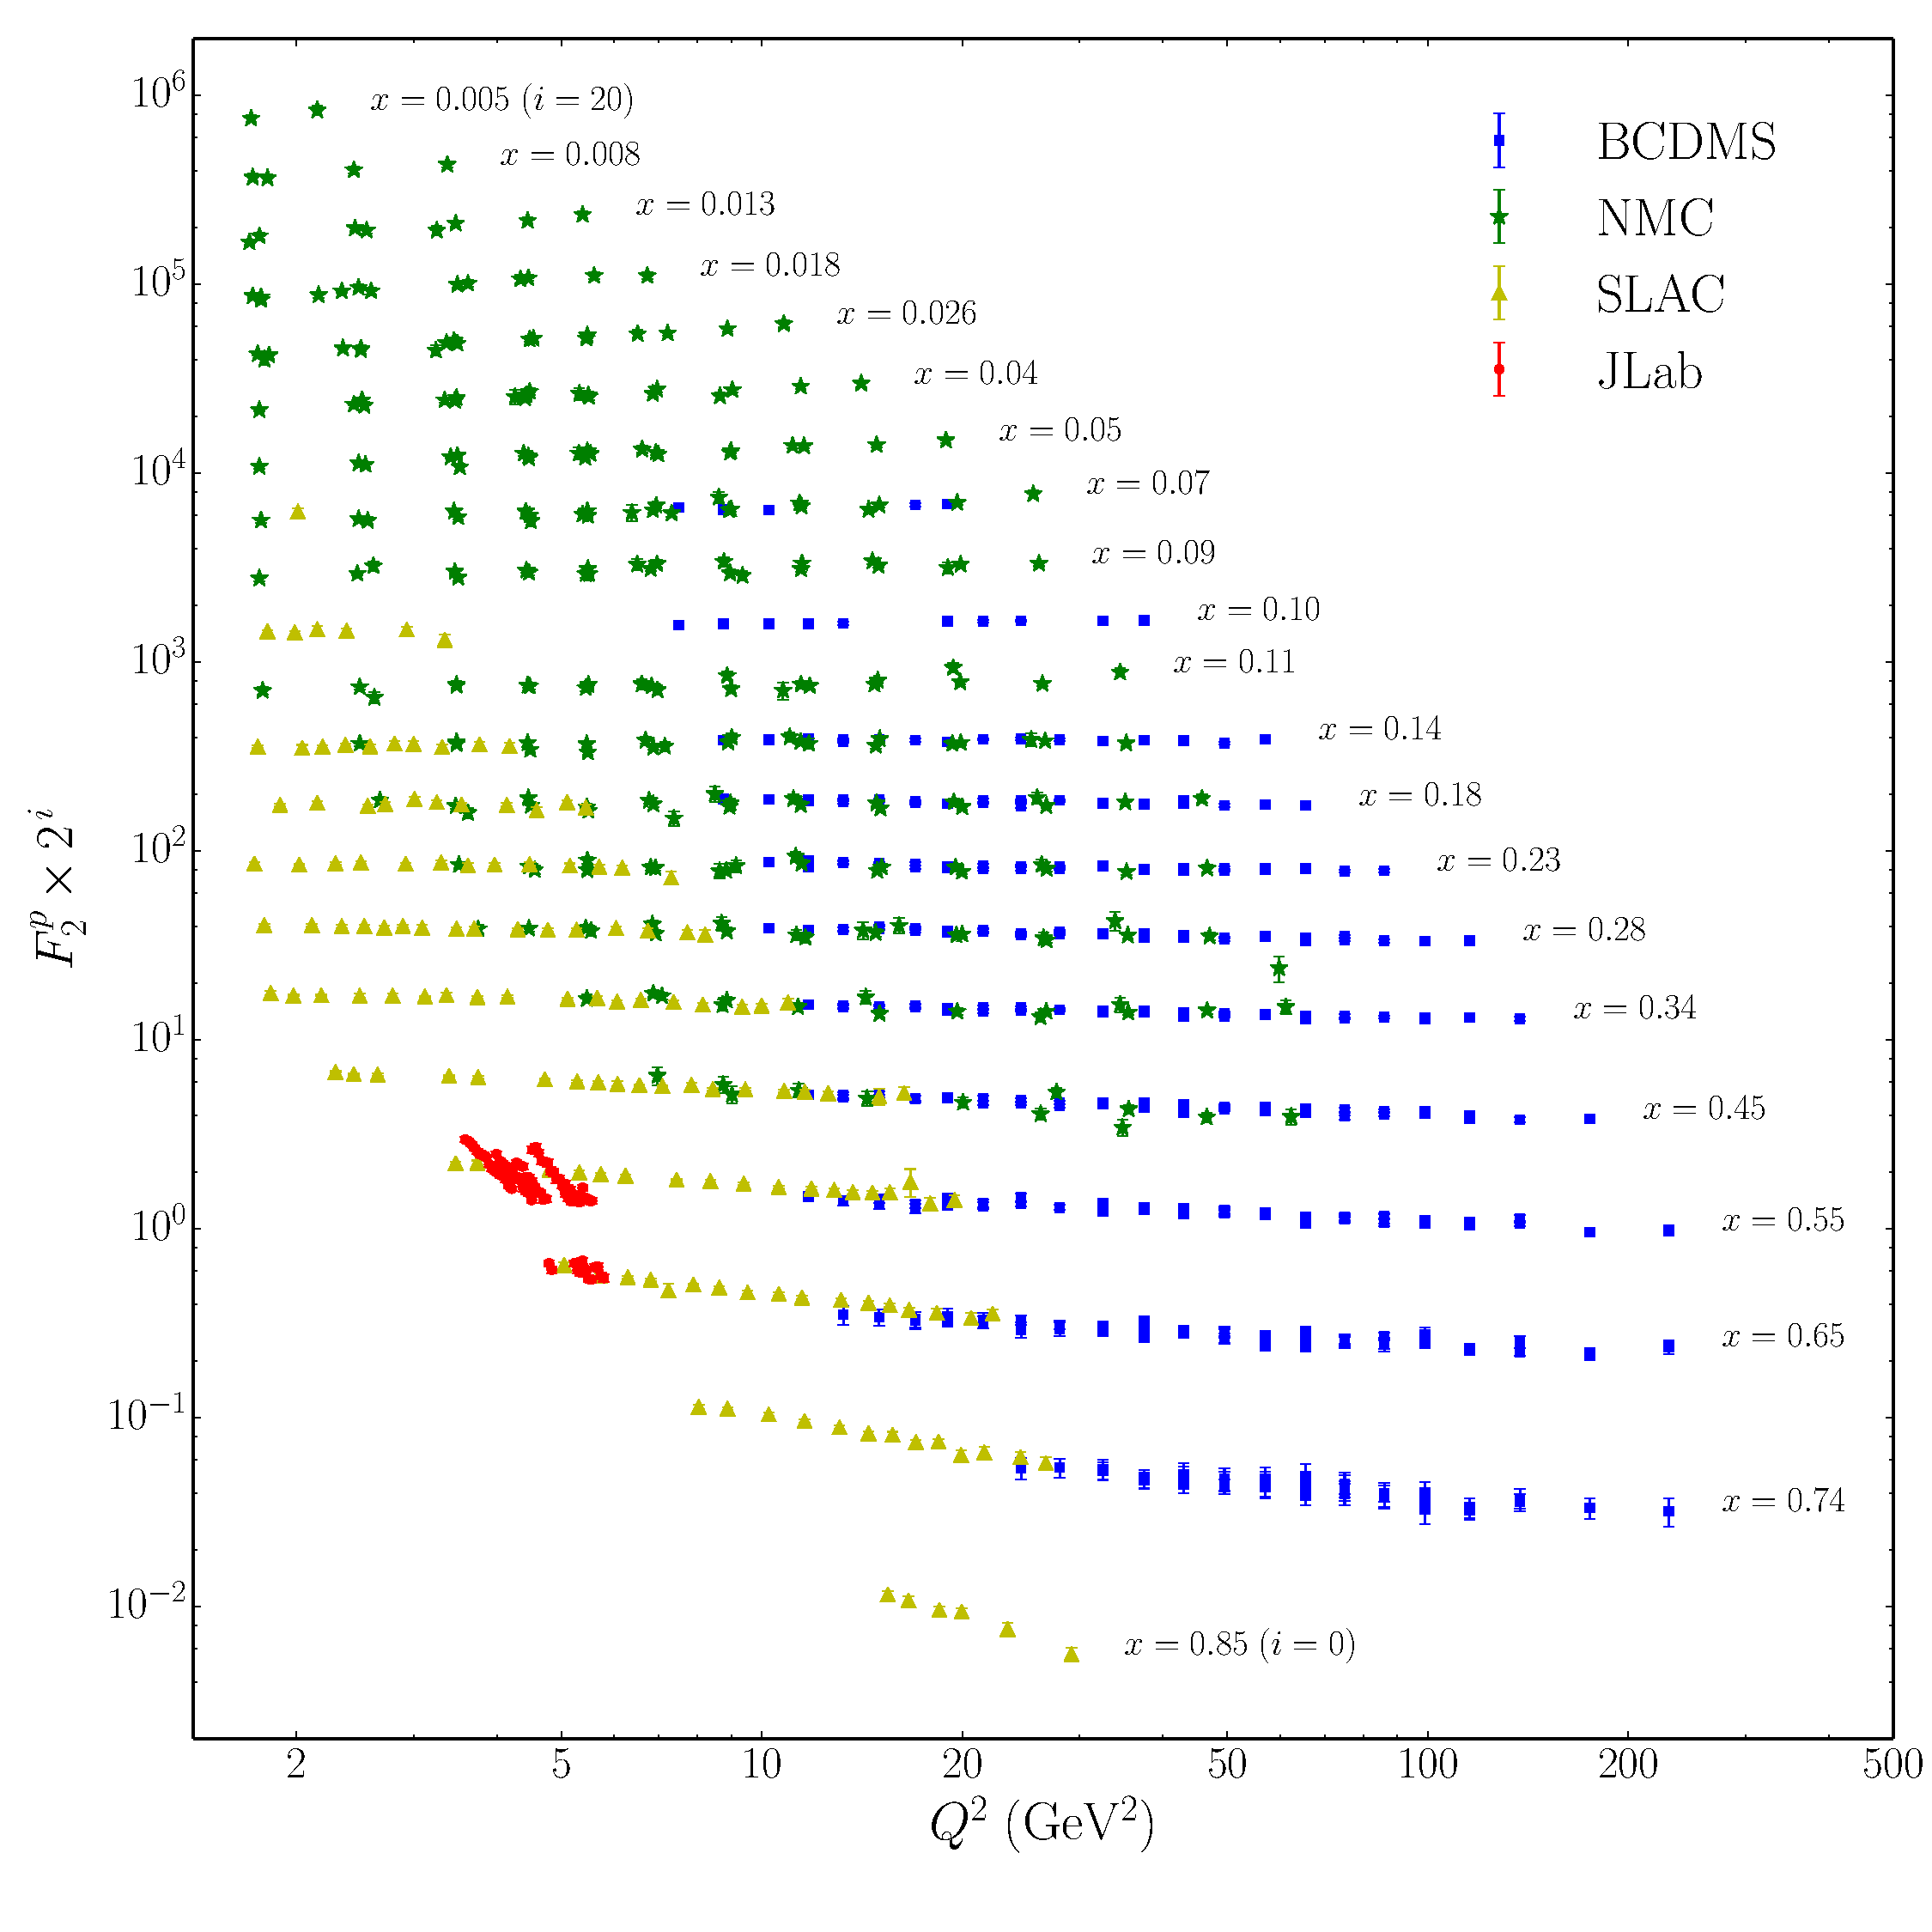
\includegraphics[width=15cm]{/u/group/cteqX/wmelnitc/CJgit/sharespace/codes/gallery/F2p.pdf}
\caption{Comparison of proton $F_2^p$ structure function data
	from BCDMS \cite{BCDMS}, NMC \cite{NMCp},
	SLAC \cite{SLAC} and JLab \cite{Malace}
	with the CJ15 NLO fit, for various $Q^2$ and $x$.
	The data at fixed $x$ values have been scaled by a factor
	$2^i$, from $i=0$ for $x=0.85$ to $i=20$ for $x=0.005$
	in steps of $i=1$.}
\label{fig:F2p}
\end{figure} 


\begin{figure}[t]
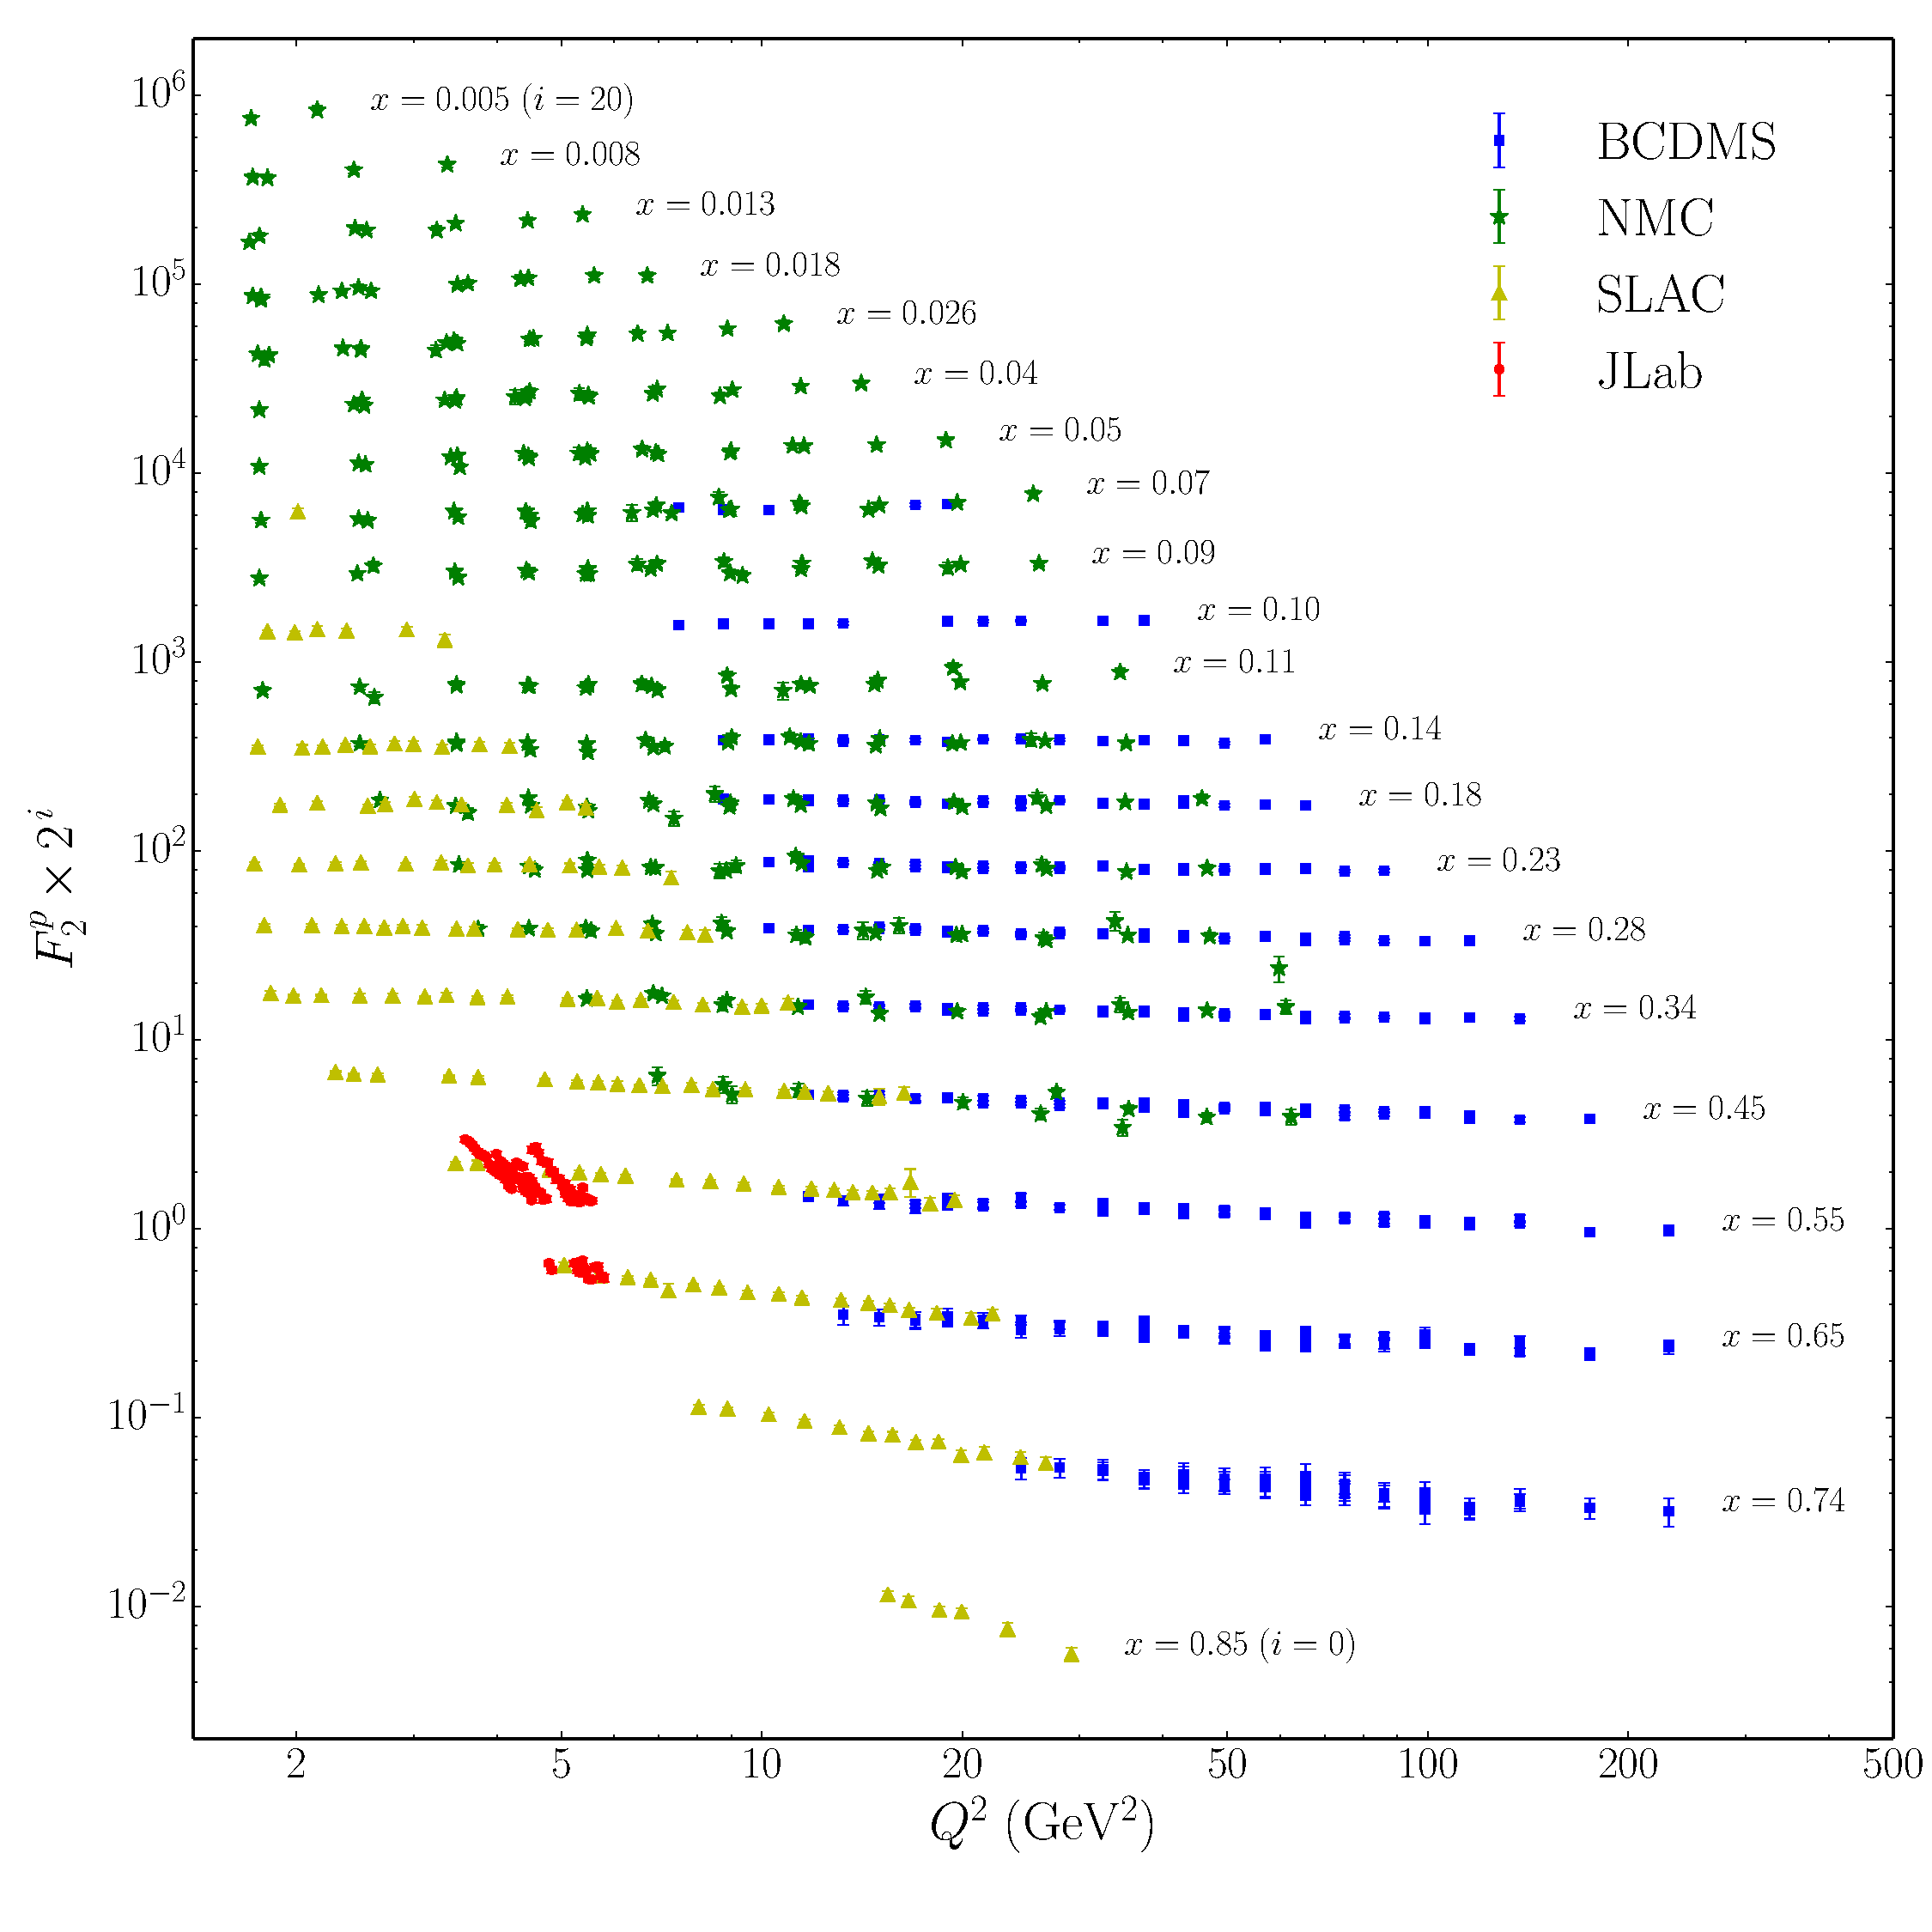
\includegraphics[width=15cm]{/u/group/cteqX/wmelnitc/CJgit/sharespace/codes/gallery/F2p.pdf}
\caption{{\color{red}[PLACEHOLDER FIGURE]...}
	As for Fig.~\ref{fig:F2p}, but for the deuteron $F_2^d$
	structure function, illustrating data from BCDMS \cite{BCDMS},
	SLAC \cite{SLAC} and JLab \cite{Malace}.
	{\color{red}...[WHAT TO DO WITH NMC $F_2^d/F_2^p$ ?]...}}
\label{fig:F2d}
\end{figure} 


\begin{figure}[t]
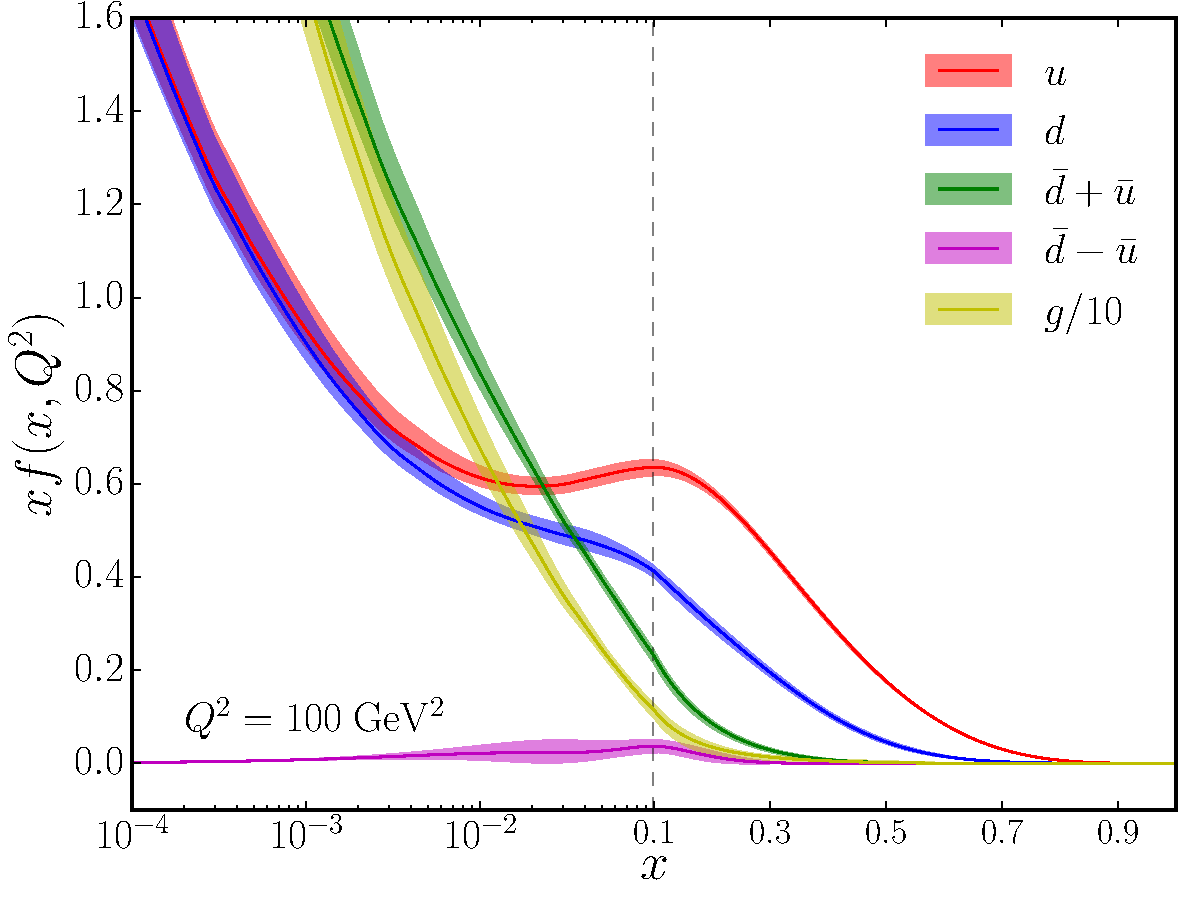
\includegraphics[width=15cm]{/u/group/cteqX/wmelnitc/CJgit/sharespace/codes/gallery/xpdf.pdf}
\caption{Comparison of CJ15 PDFs for different flavors
	($u, d, \bar d + \bar u, \bar d - \bar u$ and $g/10$)
	at a scale $Q^2=10$~GeV$^2$, for $T=1$.
	Note the combined logarithimic/linear scale along the $x$-axis.}
\label{fig:pdf}
\end{figure} 


\begin{figure}[t]
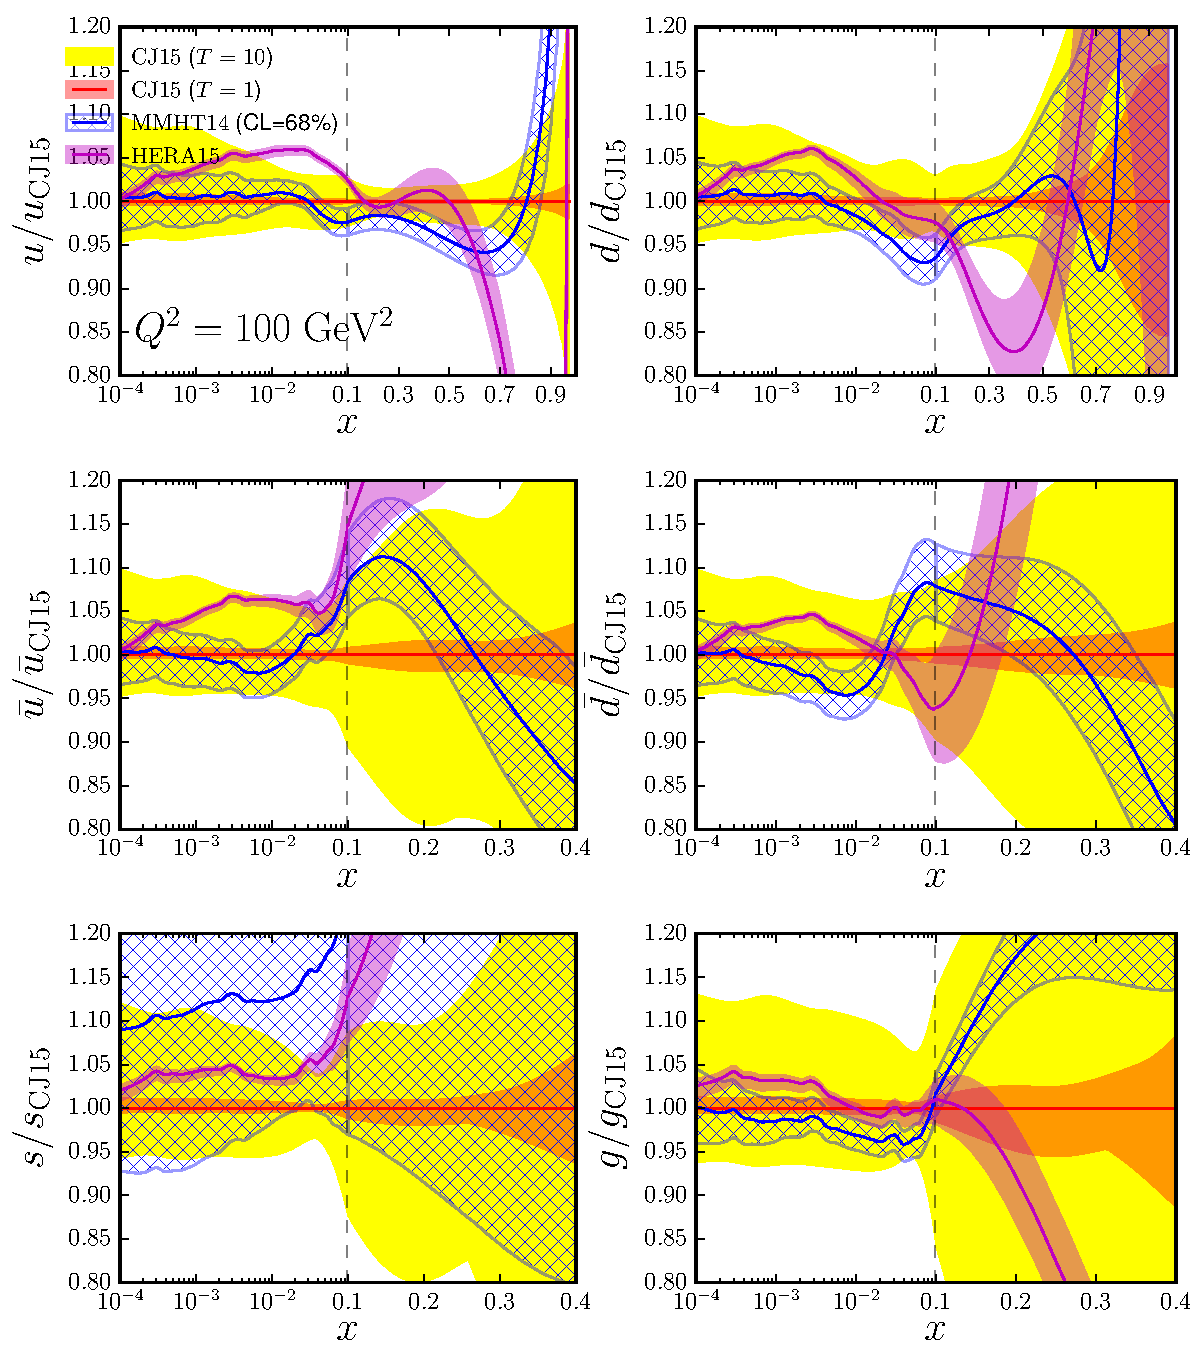
\includegraphics[width=15cm]{/u/group/cteqX/wmelnitc/CJgit/sharespace/codes/gallery/ratio.pdf}
\caption{Ratio of PDFs to the CJ15 central values for various PDF sets:
	CJ15 for tolerance $T=1$ (red) and $T=10$ (yellow),
	MMHT14 \cite{MMHT14} (blue),
	HERAPDF15 \cite{HERAPDF15} (green), and
	NNPDF3.0 \cite{NNPDF3.0} (magenta).
	Note the different scales on the vertical axes used for
	different flavors.}
\label{fig:ratio}
\end{figure} 


\begin{figure}[t]
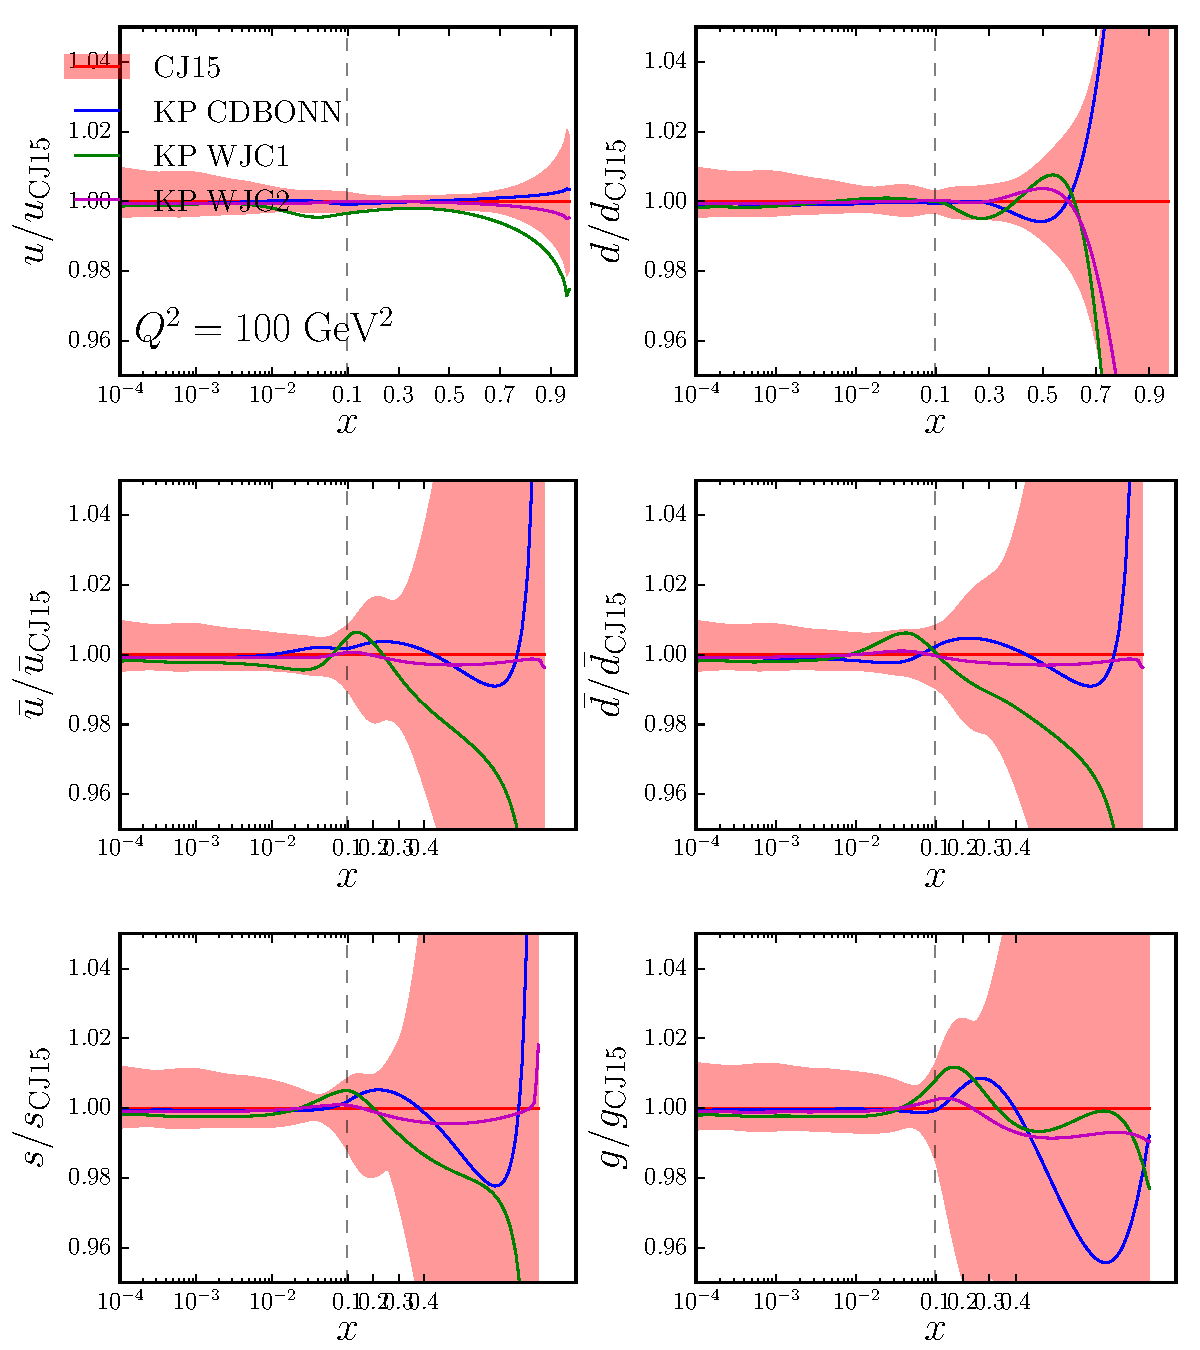
\includegraphics[width=15cm]{/u/group/cteqX/wmelnitc/CJgit/sharespace/codes/gallery/ratio_wfn.pdf}
\caption{Ratio of PDFs fitted using various deuteron wave function models
	to the CJ15 PDFs (which use the AV18 deuteron wave function):
	CD-Bonn (red solid lines),
	WJC-1 (green dashed lines),
	WJC-2 (blue solid lines).
	The CJ15 PDFs (yellow band) are shown for $T=1$, and the
	off-shell parametrization (\ref{eq:delffit}) is used for
	all cases.  Note the different scale on the vertical axes
	for the	$d$-quark and gluon distributions.}
\label{fig:ratio_wfn}
\end{figure} 


\begin{figure}[t]
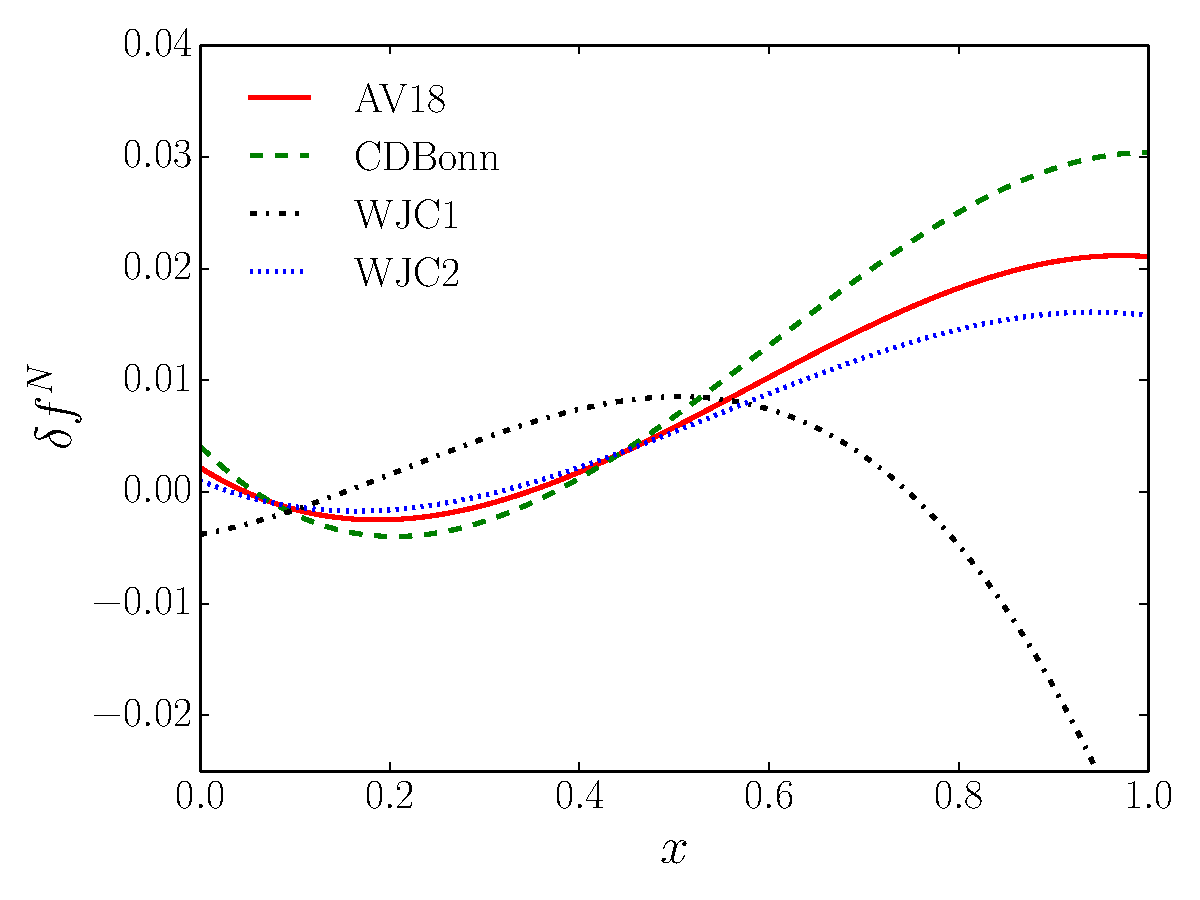
\includegraphics[width=15cm]{/u/group/cteqX/wmelnitc/CJgit/sharespace/codes/gallery/off_shell.pdf}
\caption{Fitted nucleon off-shell correction $\delta f^N$ for the
	parametrization in Eq.~(\ref{eq:delffit}), using the
	AV18 (solid red line), CD-Bonn (dashed green line),
	WJC-1 (dot-dashed black line) and WJC-2 (dotted blue line)
	wave functions.}
\label{fig:off_shell}
\end{figure} 


\begin{figure}[t]
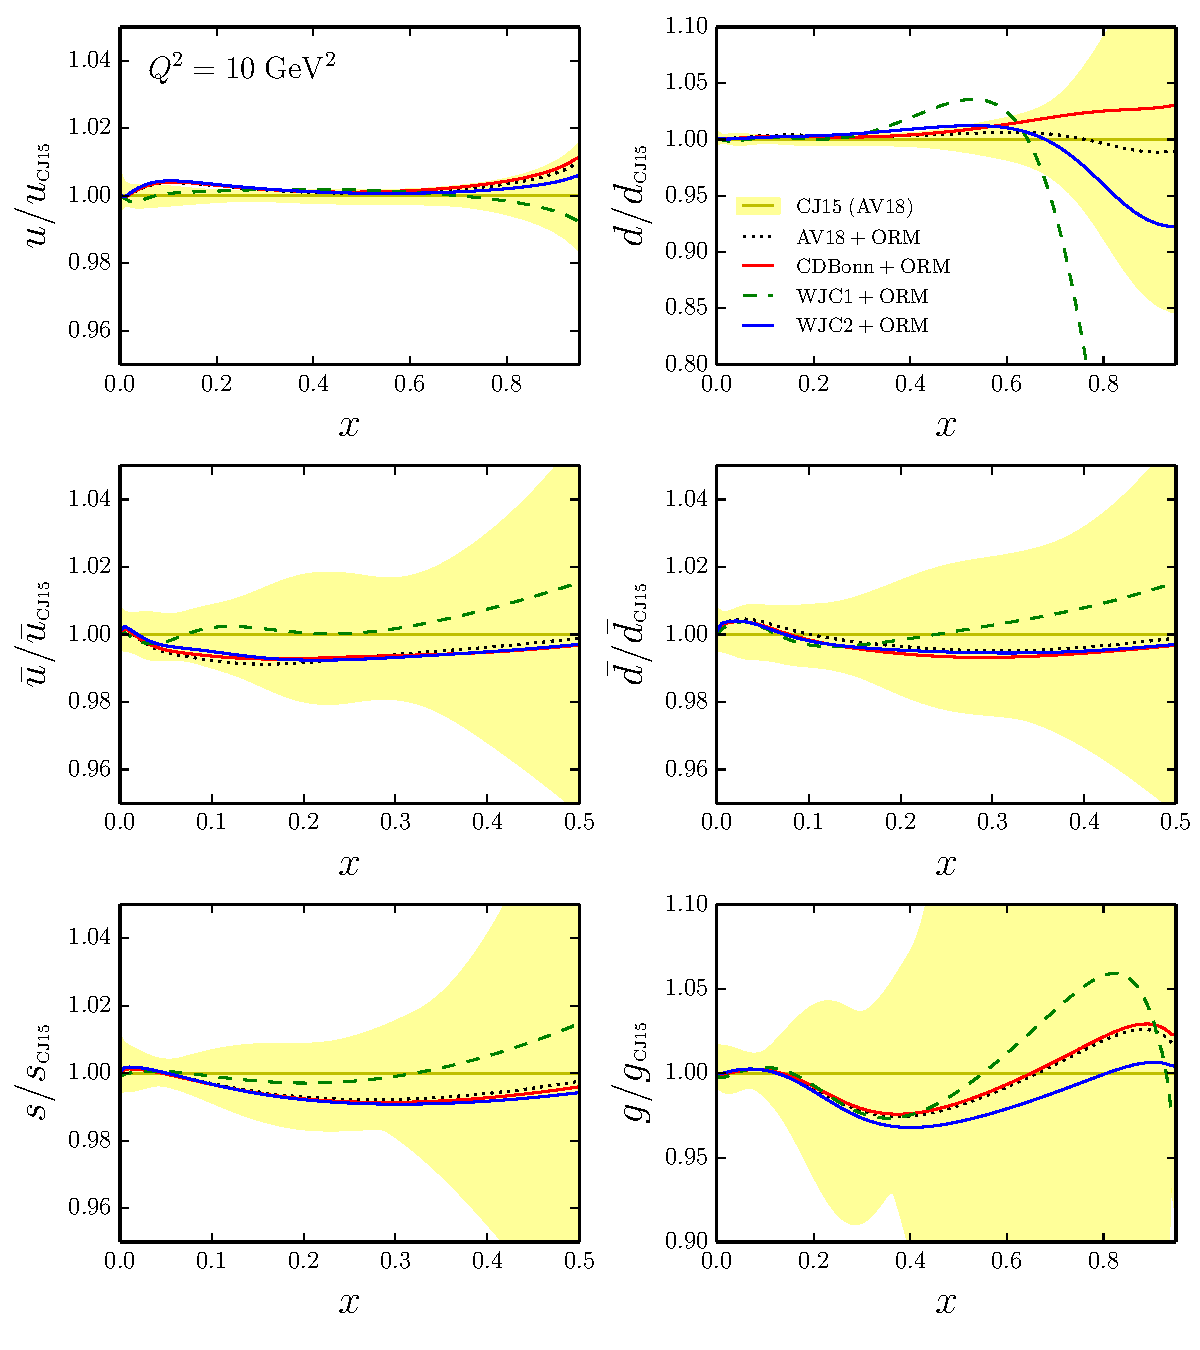
\includegraphics[width=15cm]{/u/group/cteqX/wmelnitc/CJgit/sharespace/codes/gallery/ratio_off.pdf}
\caption{Ratio of PDFs computed using the off-shell covariant spectator
	(OCS) model and different deuteron wave functions to the CJ15
	PDFs (which use the off-shell parametrization (\ref{eq:delffit})
	and the AV18 deuteron wave function):
	OCS model with the AV18 wave function (black dotted lines),
	CD-Bonn (red solid lines),
	WJC-1 (green dashed lines), and
	WJC-2 (blue solid lines).
	Note the different scale on the vertical axes for the
	$d$-quark and gluon distributions.}
\label{fig:ratio_off}
\end{figure} 


\begin{figure}[t]
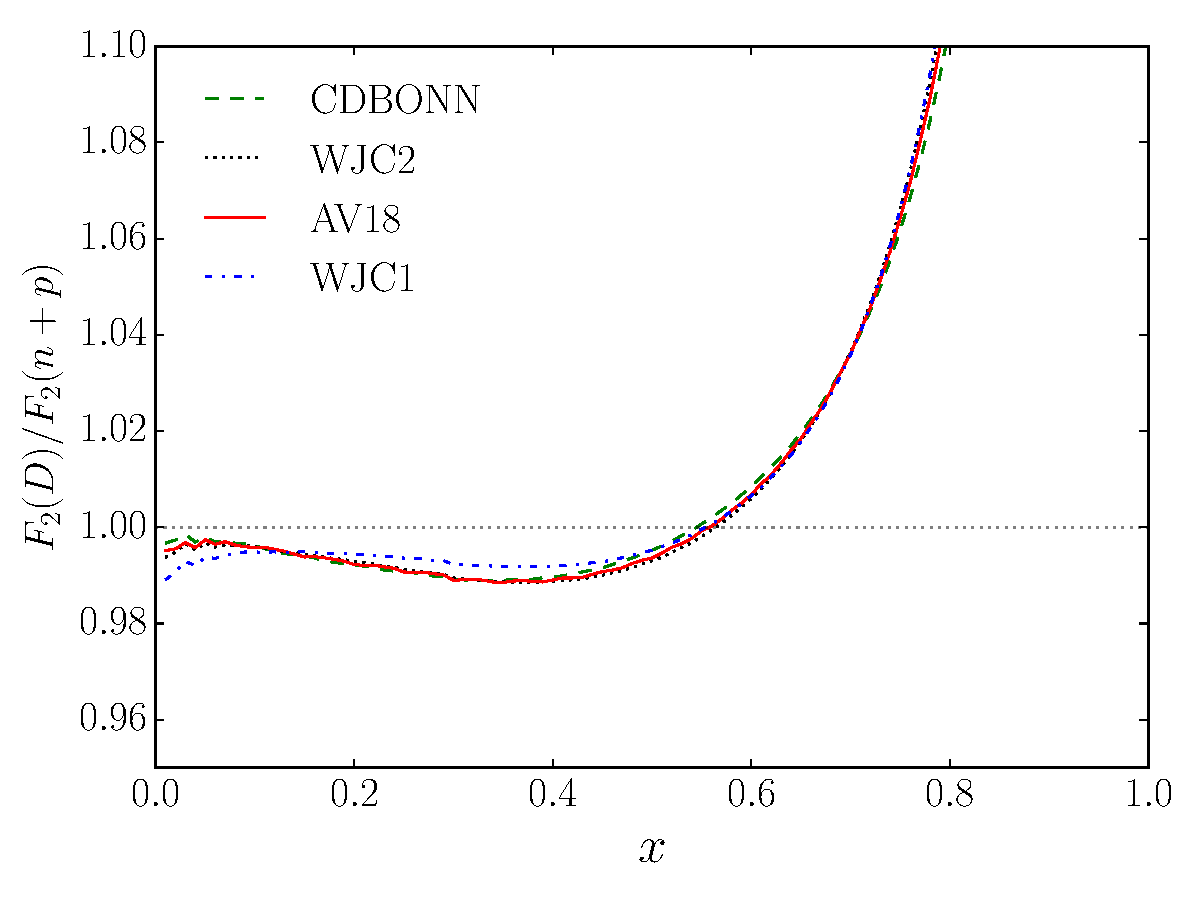
\includegraphics[width=15cm]{/u/group/cteqX/wmelnitc/CJgit/sharespace/codes/gallery/F2d_F2_I.pdf}
\caption{Ratio of deuteron to isoscalar nucleon structure functions
	$F_2^d/F_2^N$ for different deuteron wave function models
	at $Q^2=10$~GeV$^2$.
	{\color{red} ...[SMOOTH CURVES]...}}
\label{fig:F2dN}
\end{figure}


\begin{figure}[t]
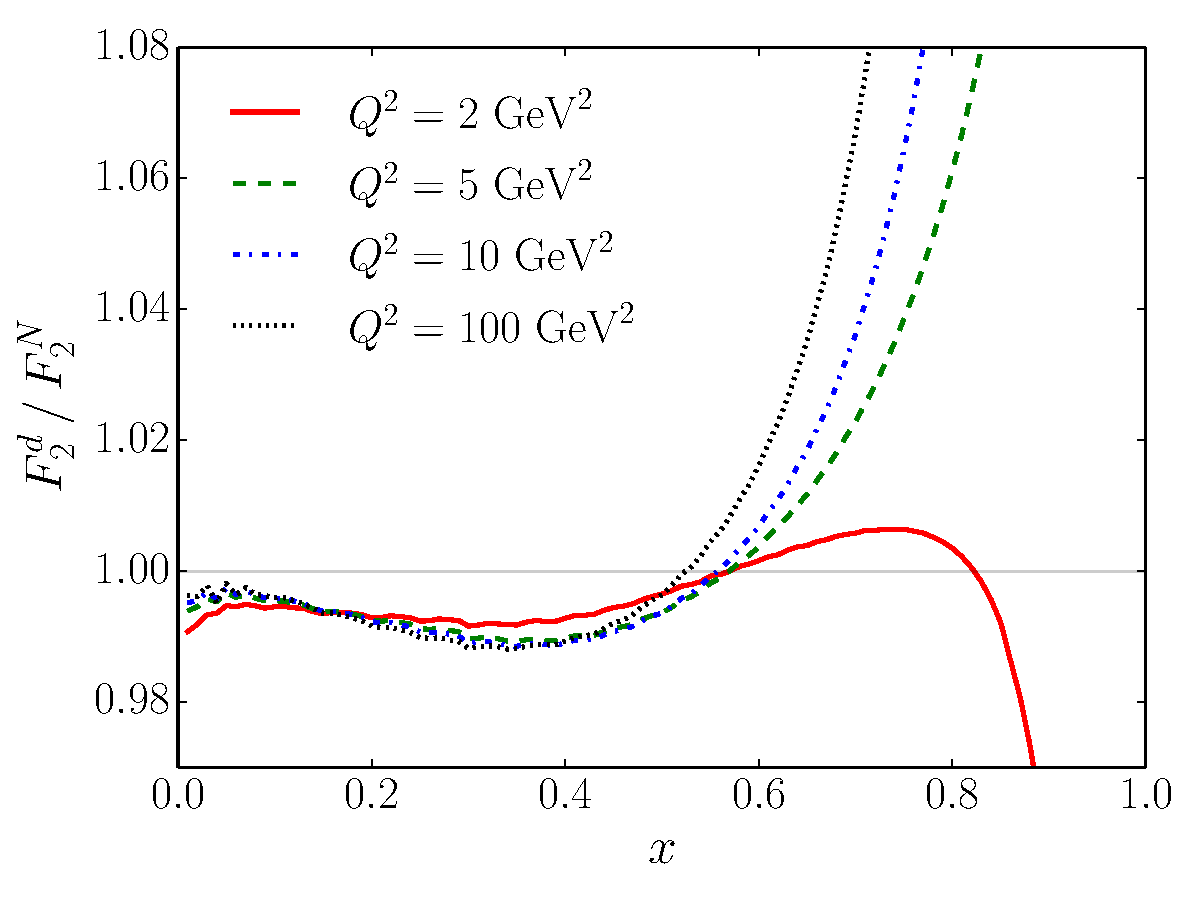
\includegraphics[width=15cm]{/u/group/cteqX/wmelnitc/CJgit/sharespace/codes/gallery/F2d_F2_II.pdf}
\caption{Ratio of deuteron to isoscalar nucleon structure functions
	$F_2^d/F_2^N$ computed from the CJ15 PDFs for different
	values of $Q^2$.
	{\color{red} ...[SMOOTH CURVES]...}}
\label{fig:F2dN_Q2}
\end{figure}


\begin{figure}[t]
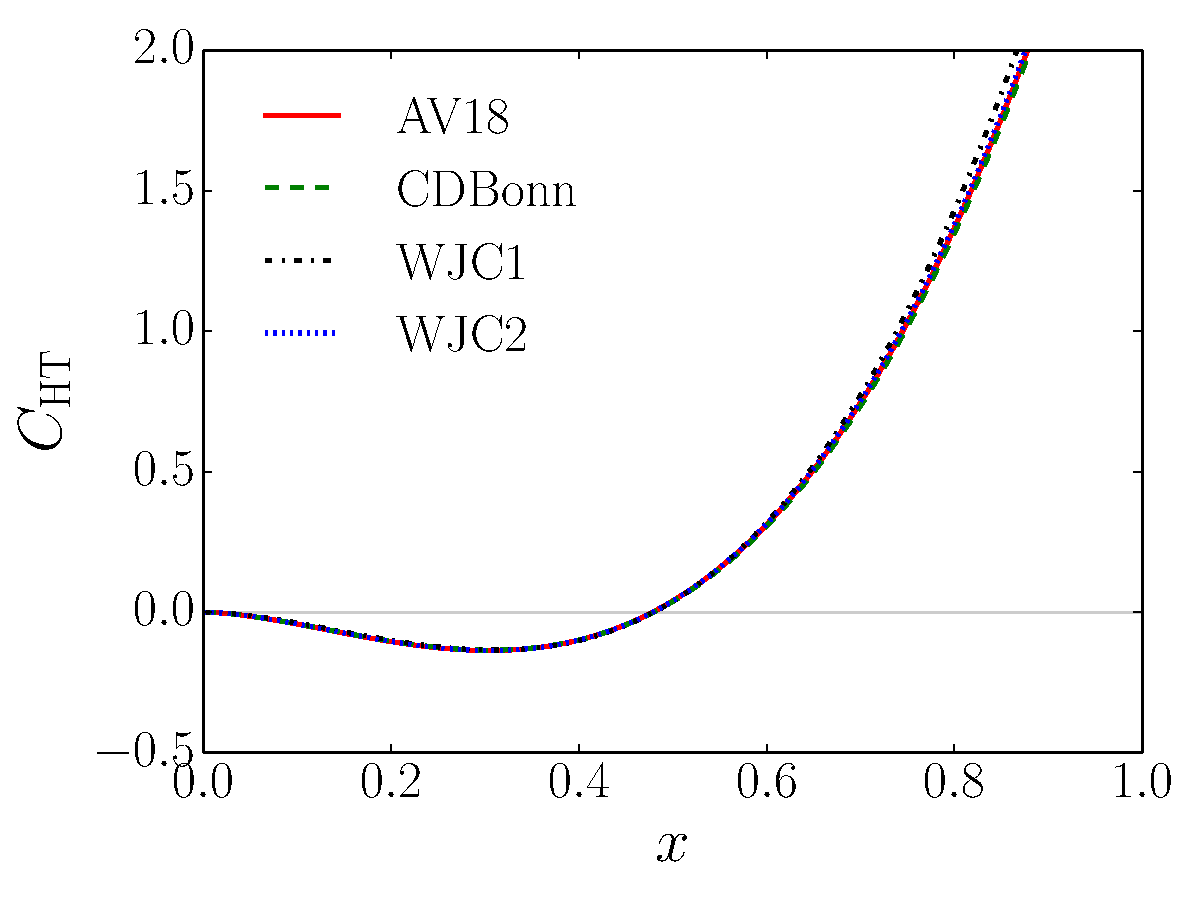
\includegraphics[width=15cm]{/u/group/cteqX/wmelnitc/CJgit/sharespace/codes/gallery/ht.pdf}
\caption{Fitted higher twist function $C_{\rm HT}$ from
	Eq.~(\ref{eq:C_ht}), in units of GeV$^2$, for different
	deuteron wave function models.}
\label{fig:Cht}
\end{figure}


\begin{figure}[t]
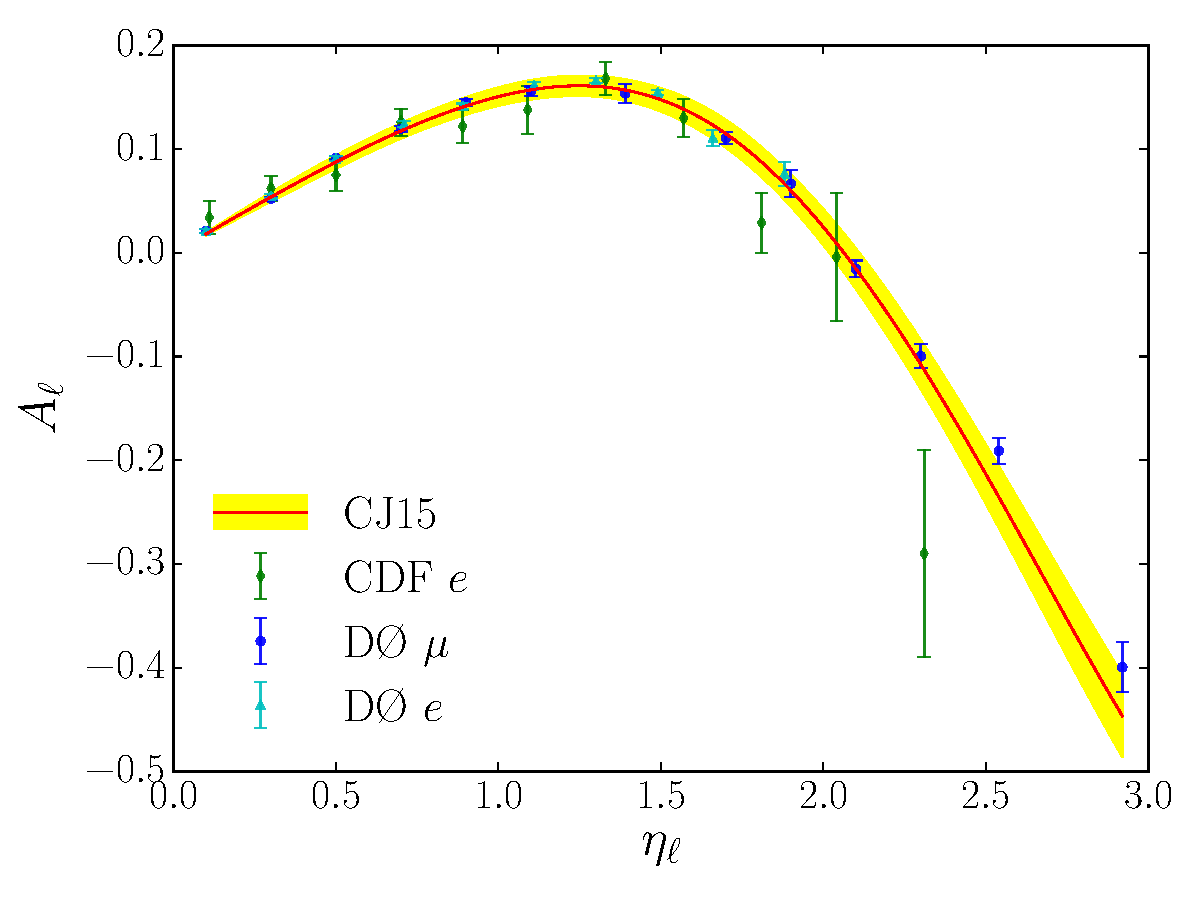
\includegraphics[width=15cm]{/u/group/cteqX/wmelnitc/CJgit/sharespace/codes/gallery/Lasy.pdf}
\caption{Lepton charge asymmetry $A_{\ell}$ from
	$p\bar p \to W X \to \ell \nu X$ as a function of the
	lepton pseudorapidity $\eta_{\ell}$ from
	CDF electron (green diamonds) \cite{CDF_e}, and
	D\O\ muon (blue circles) \cite{D0_mu} and
	electron (cyan triangles) \cite{D0_e} data
	compared with the CJ15 fit.}
\label{fig:Lasy}
\end{figure} 

  
\begin{figure}[t]
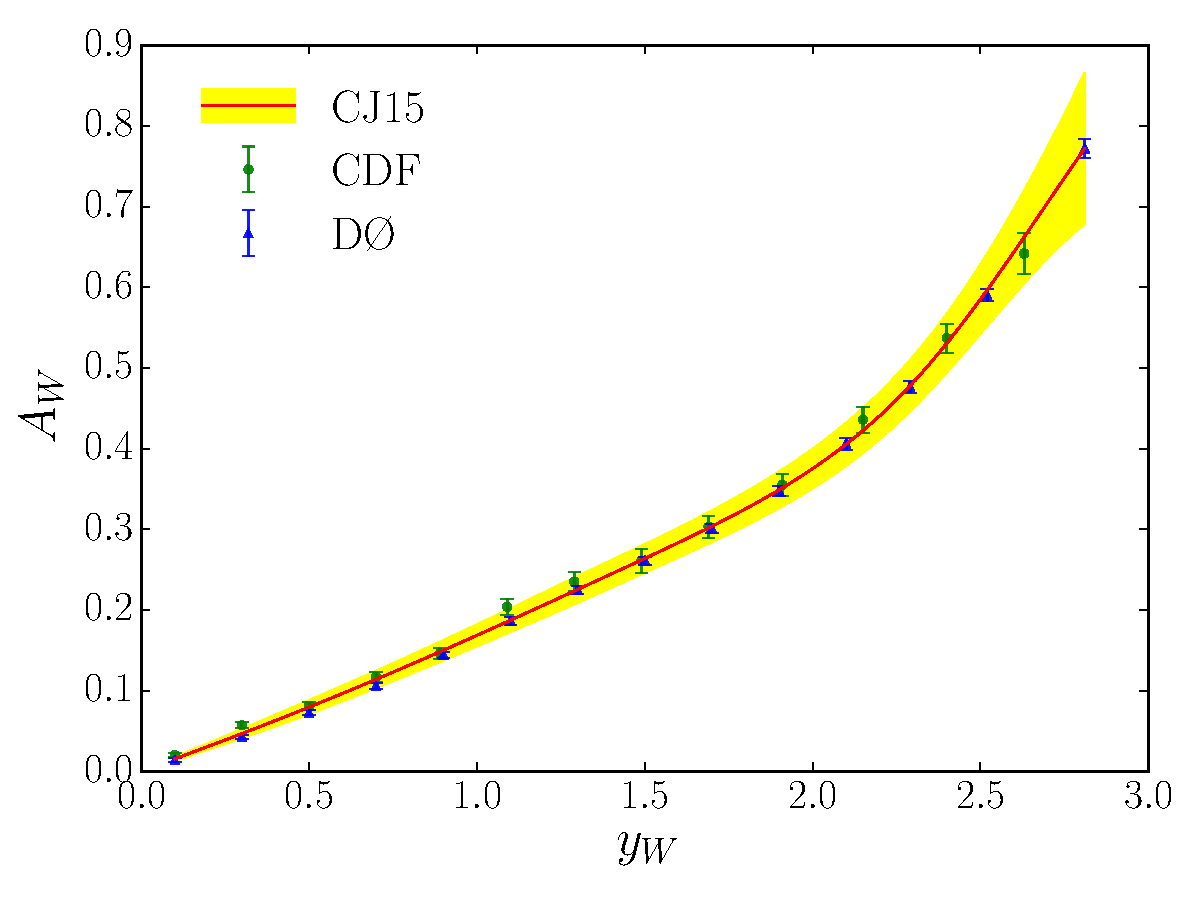
\includegraphics[width=15cm]{/u/group/cteqX/wmelnitc/CJgit/sharespace/codes/gallery/Wasy.pdf}
\caption{$W$ boson charge asymmetry $A_W$ from $p\bar p \to W X$
	as a function of the $W$ boson rapidity $y_W$ for
	CDF (green circles) \cite{CDF_W} and
	D\O\ (blue triangles) \cite{D0_W} data
	compared with the CJ15 fit.}
\label{fig:Wasy}
\end{figure} 


\begin{figure}[t]
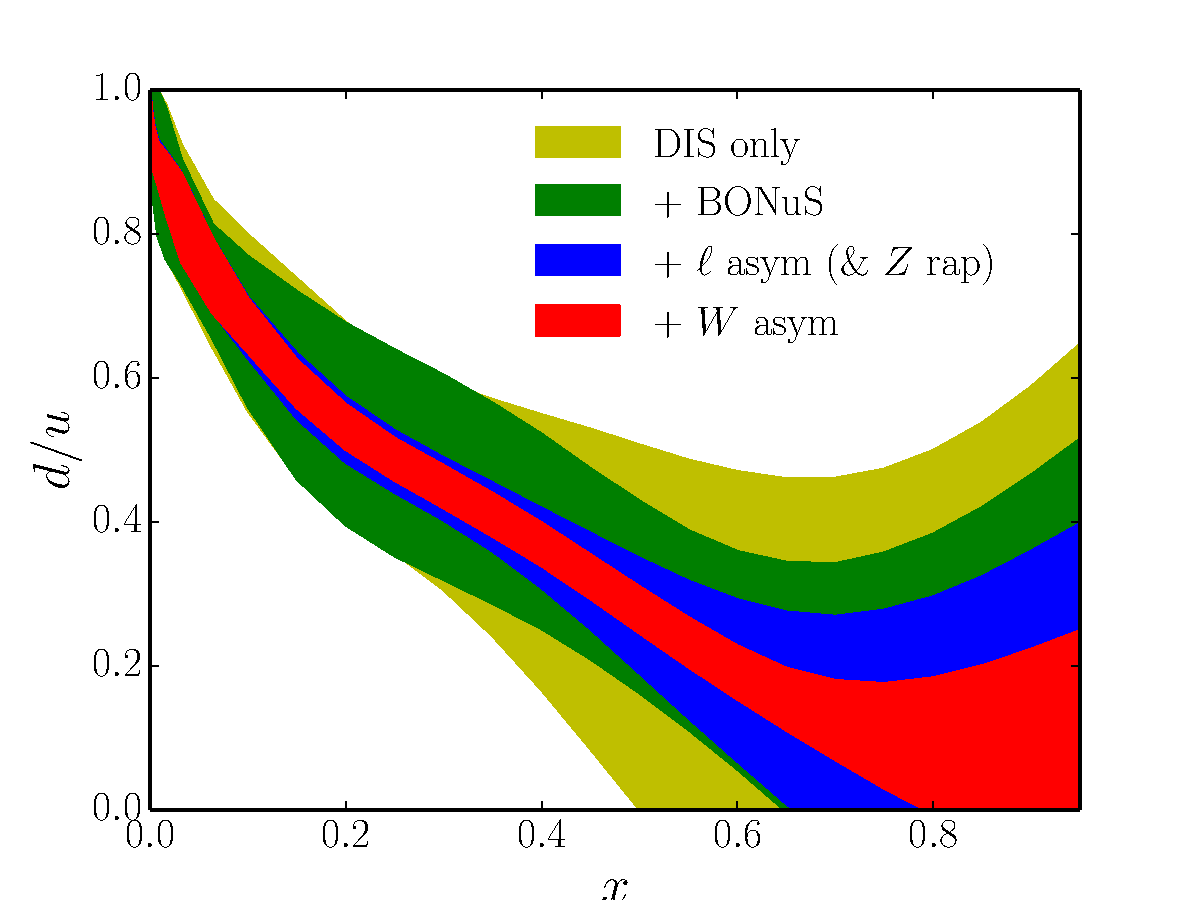
\includegraphics[width=15cm]{/u/group/cteqX/wmelnitc/CJgit/sharespace/codes/gallery/du_data.pdf}
\caption{Impact of various data sets on the $d/u$ ratio at
	$Q^2=10$~GeV$^2$. The uncertainty band is largest for the
	  DIS only data (yellow band),
	and decreases with the successive addition of
	  JLab $F_2^n/F_2^d$ \cite{BONuS} data (green band),
	  lepton asymmetry \cite{CDF_e, D0_mu, D0_e}
	(and $Z$ rapidity \cite{CDFZ, D0Z}) data (blue band), and
	  $W$ boson asymmetry data \cite{CDF_W, D0_W} (red band).
	{\color{red}...[FIGURE NEEDS SMOOTHING]...}}
\label{fig:du_data}
\end{figure} 


\begin{figure}[t]
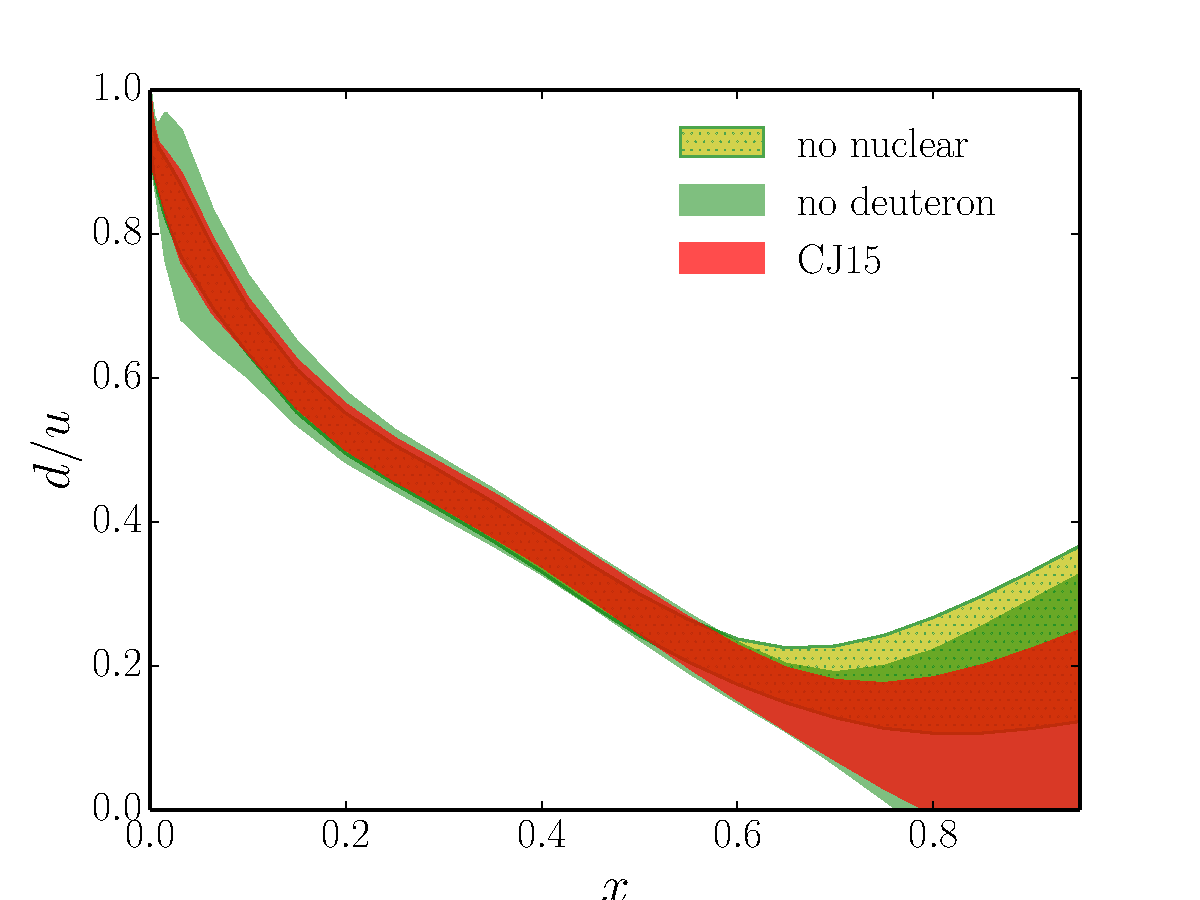
\includegraphics[width=15cm]{/u/group/cteqX/wmelnitc/CJgit/sharespace/codes/gallery/du_nuc.pdf}
\caption{Impact on the CJ15 $d/u$ ratio (red band) of removing the
	deuterium nuclear corrections (yellow shaded band),
	and omitting the deuterium data (green band).
	{\color{red}...[FIGURE NEEDS SMOOTHING]...}}
\label{fig:du_nuc}
\end{figure} 


\begin{figure}[t]
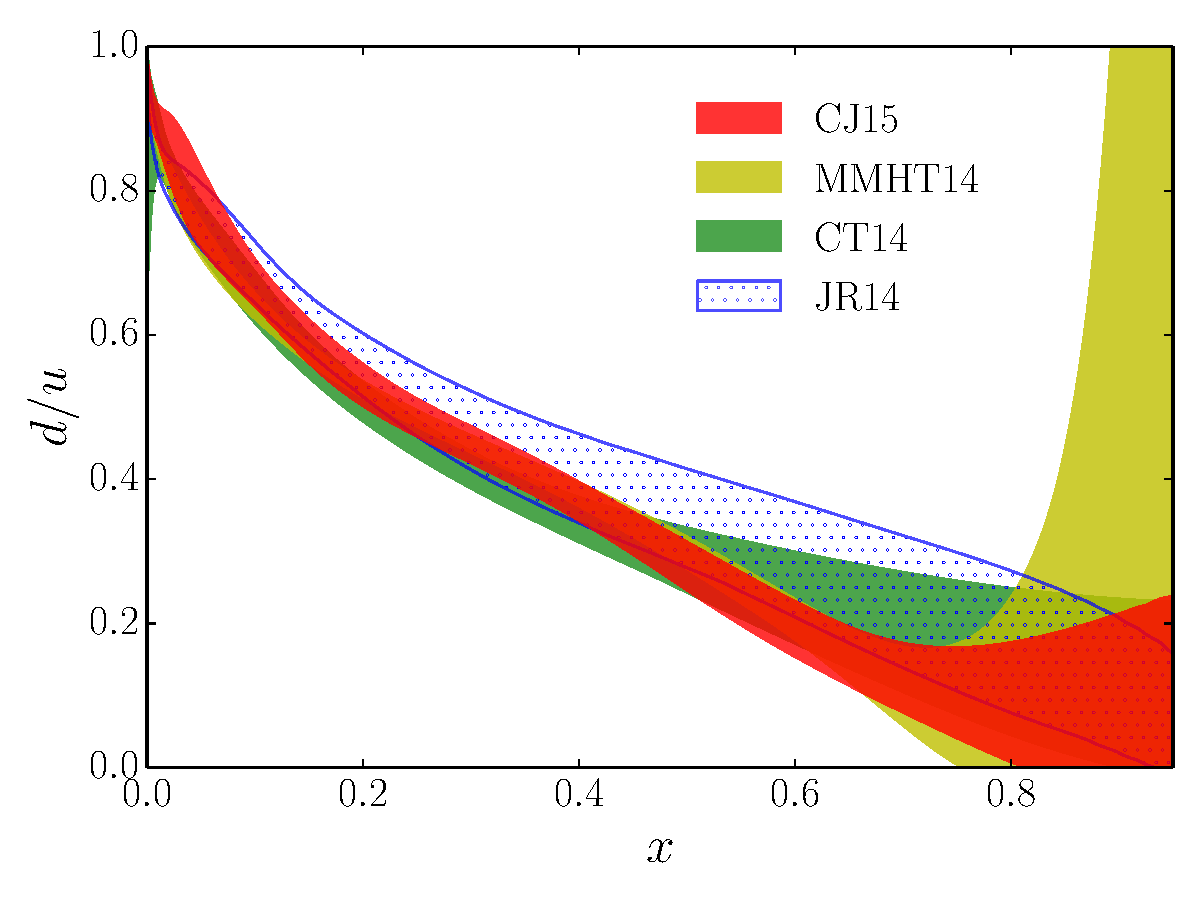
\includegraphics[width=15cm]{/u/group/cteqX/wmelnitc/CJgit/sharespace/codes/gallery/du_pdfs.pdf}
\caption{Comparison of the $d/u$ ratio at $Q^2=10$~GeV$^2$ for different
	PDF parametrizations:
	CJ15 (red band),
	MMHT14 \cite{MMHT14} (yellow band),
	CT14 \cite{CT14} (green band), and
	JR14 \cite{JR14} (blue dotted band).}
\label{fig:du_pdfs}
\end{figure} 


\newpage
%%%%%%%%%%%%%%%%%%%%%%%%%%%%%%%%%%%%%%%%%%%%%%%%%%%%%%%%%%%%%%%%%%%%
\begin{table}[t]
\caption{Data sets used in the CJ15 NLO global analysis (which uses
	the AV18 deuteron wave function and off-shell parametrization
	in Eq.~(\ref{eq:delffit}), with the corresponding number of
	data points and the respective $\chi^2$ values for each set.
	For comparison the $\chi^2$ for the LO fit and for an NLO
	fit with the OCS off-shell model are also given.
	{\color{red} ...[remove LO \& OCS entries?]...} \\}
\centering
{\scriptsize  
\begin{tabular}[c]{llrrrr}  \hline
  & experiment  & \# points\!\!\!\! & \multicolumn{3}{c}{\ \ \ \ \ $\chi^2$} \\
  & 		& 		    & NLO  & LO  & NLO (OCS) \\ \hline
DIS $F_2$
  & BCDMS $(p)$ 	\cite{BCDMS}    & 351 & 437 & 432 & 435 \\
  & BCDMS $(d)$ 	\cite{BCDMS}    & 254 & 294 & 299 & 289 \\
  & NMC   $(p)$   	\cite{NMCp}     & 275 & 407 & 414 & 406 \\
  & NMC   $(d/p)$ 	\cite{NMCdop}   & 189 & 172 & 180 & 173 \\
  & SLAC  $(p)$  	\cite{SLAC}     & 564 & 435 & 496 & 436 \\
  & SLAC  $(d)$  	\cite{SLAC}     & 582 & 372 & 417 & 386 \\
  & JLab  $(p)$  	\cite{Malace}   & 136 & 166 & 164 & 166 \\
  & JLab  $(d)$  	\cite{Malace}   & 136 & 124 & 127 & 123 \\
  & JLab  $(n/d)$	\cite{BONuS}  	& 191 & 217 & 224 & 215 \\
DIS $\sigma$
  & HERA (NC $e^-p$) 	\cite{HERA1}    & 145 & 112 & 161 & 113 \\
  & HERA (NC $e^+p$) 	\cite{HERA1}    & 408 & 541 & 872 & 541 \\
  & HERA (CC $e^-p$) 	\cite{HERA1}    &  34 &  19 &  19 &  19 \\
  & HERA (CC $e^+p$) 	\cite{HERA1}    &  34 &  31 &  33 &  32 \\
Drell-Yan
  & E605 $(p{\rm Cu})$	\cite{E605}     & 119 &  93 & 104 &  93 \\ % p-Cu data
  & E866 $(pp)$		\cite{E866}     & 121 & 139 & 155 & 139 \\
  & E866 $(pd)$ 	\cite{E866}     & 129 & 144 & 191 & 144 \\
  & E866 $(pd/pp)$ 	\cite{E866rat}  &  12 &   9 &   9 &   8 \\
$W/$charge asymmetry
  & CDF  ($e$)		\cite{CDF_e}    &  11 &  12 &  11 &  12 \\
  & D\O\ ($\mu$)  	\cite{D0_mu}    &  10 &  20 &  21 &  29 \\  
  & D\O\ ($e$) 		\cite{D0_e}     &  13 &  27 &  56 &  22 \\
  & CDF  ($W$)    	\cite{CDF_W}    &  13 &  15 &  12 &  15 \\
  & D\O\ ($W$)    	\cite{D0_W}     &  14 &  16 &  47 &  16 \\
$Z$ rapidity
  & CDF  ($Z$)		\cite{CDFZ}     &  28 &  27 &  79 &  28 \\ 
  & D\O\ ($Z$)		\cite{D0Z}      &  28 &  16 &  23 &  16 \\
jet
  & CDF  (run 2)       	\cite{CDFjet2}  &  72 &  15 &  22 &  15 \\
  & D\O\ (run 2)       	\cite{D0jet2}   & 110 &  21 &  46 &  22 \\
$\gamma$+jet
  & D\O\ 1           	\cite{D0gamjet} &  16 &   6 &  20 &   6 \\    
  & D\O\ 2           	\cite{D0gamjet} &  16 &  15 &  40 &  15 \\
  & D\O\ 3           	\cite{D0gamjet} &  12 &  25 &  35 &  25 \\
  & D\O\ 4           	\cite{D0gamjet} &  12 &  13 &  77 &  13 \\ \hline
%
total        		&		& 4035 &\ \ \ \ {\bf 3941} & 4786 & 3952 \\
total + norm 		&		&      &\ \ \ \ {\bf 3950} & 4918 & 3961 \\ \hline
$\chi^2/{\rm dof}$	&		&      & {\bf 0.979} & 1.219 & 0.982 \\  \hline\\
%
\end{tabular}
}
\label{tab:chi2}
\end{table}


\begin{table}[t]
\begin{center}
\caption{Leading twist parameter values for the
	$u_v$, $d_v$, $\bar d+\bar u$, $\bar d-\bar u$ and $g$ PDFs
	[Eq.~(\ref{eq:param})] from the CJ15 NLO analysis at the
	initial scale $Q_0$~GeV.  Parameters without errors have
	been fixed.  For the strange to non-strange sea quark PDF
	ratio [Eq.~(\ref{eq:kappa})], we take $\kappa=0.4$.
	(The parameter values are given to 5 significant figures
	to avoid rounding errors.)
	{\color{red} ...[make neater/reduce sig. figs?]...} \\}
{\scriptsize
\begin{tabular}{c|ccccc}\hline
parameter	& $u_v$
		& $d_v$
		& $\bar d+\bar u$
		& $\bar d-\bar u$
		& $g$				\\ \hline
$a_0$		& 2.3585
		& 23.233
		& 0.14121 $\pm$ 0.0050459
		& 35712
		& 46.706			\\
$a_1$		& 0.60985 $\pm$ 0.020299
		& 1.1387 $\pm$ 0.034586
		& $-0.21785 \pm 0.0039454$
		& 3.9867 $\pm$ 0.049301
		& 0.61586 $\pm$ 0.038277	\\
$a_2$		& 3.5377 $\pm$ 0.011405
		& 6.6180 $\pm$ 0.15977
		& 8.4003 $\pm$ 0.14833
		& 20.289 $\pm$ 0.66322
		& 6.2335 $\pm$ 1.1222		\\
$a_3$		& 0
		& $-3.5743 \pm 0.090782$
		& 0
		& 17
		& $-3.2703 \pm 0.16746$		\\		
$a_4$		& 3.5169 $\pm$ 0.42791
		& 4.9133 $\pm$ 0.14586
		& 16.055 $\pm$ 1.1403
		& 49.881 $\pm$ 7.1398
		& 3.0338 $\pm$ 0.31300		\\
$b$		& ---
		& 0.0042424 $\pm$ 0.00070691
		& ---
		& ---
		& ---				\\
$c$		& ---
		& 2
		& ---
		& ---
		& ---				\\ \hline
\end{tabular}
}
\label{tab:LTparams}
\end{center}
\end{table}


\begin{table}[h]
\begin{center}
\caption{Parameter values for the nucleon off-shell
	[Eq.~(\ref{eq:delffit})] and higher twist
	[Eq.~(\ref{eq:C_ht})] corrections to $F_2$ from
	the CJ15 NLO analysis at the input scale $Q_0^2$.
	The off-shell parameters are fitted using the
	AV18 deuteron wave function.
	Parameters without errors have been fixed.
	(The parameter values are given to 5 significant
	figures to avoid rounding errors.) \\}
{\scriptsize
\begin{tabular}{c|c}\hline
parameter	& value				\\ \hline
$C_0$ 		& 0.098222 $\pm$ 0.028518	\\
$x_0$ 		& 0.34487  $\pm$ 0.91982	\\
$x_1$		& 0.048				\\ \hline
%
$h_0$		& $-3.0094 \pm 0.24080$		\\    
$h_1$ 		& $ 1.7526 \pm 0.10135$         \\       
$h_2$ 		& $-2.0895 \pm 0.026853$        \\ \hline
\end{tabular}
}
\label{tab:other_params}
\end{center}
\end{table}


\end{document}
